% Created 2021-11-16 Tue 20:52
% Intended LaTeX compiler: pdflatex
\documentclass[11pt]{article}
\usepackage[utf8]{inputenc}
\usepackage[T1]{fontenc}
\usepackage{graphicx}
\usepackage{longtable}
\usepackage{wrapfig}
\usepackage{rotating}
\usepackage[normalem]{ulem}
\usepackage{amsmath}
\usepackage{amssymb}
\usepackage{capt-of}
\usepackage{hyperref}
\graphicspath{{../../books/}}
\DeclareMathOperator{\Max}{Max}
\DeclareMathOperator{\Adj}{Adj}
% wrong resolution of image
% https://tex.stackexchange.com/questions/21627/image-from-includegraphics-showing-in-wrong-image-size?rq=1

%%%%%%%%%%%%%%%%%%%%%%%%%%%%%%%%%%%%%%
%% TIPS                                 %%
%%%%%%%%%%%%%%%%%%%%%%%%%%%%%%%%%%%%%%
% \substack{a\\b} for multiple lines text
% \usepackage{expl3}
% \expandafter\def\csname ver@l3regex.sty\endcsname{}
% \usepackage{pkgloader}
\usepackage[utf8]{inputenc}

% nfss error
% \usepackage[B1,T1]{fontenc}
\usepackage{fontspec}

% \usepackage[Emoticons]{ucharclasses}
\newfontfamily\DejaSans{DejaVu Sans}
% \setDefaultTransitions{\DejaSans}{}

% pdfplots will load xolor automatically without option
\usepackage[dvipsnames]{xcolor}

%                                                             ┳┳┓   ┓
%                                                             ┃┃┃┏┓╋┣┓
%                                                             ┛ ┗┗┻┗┛┗
% \usepackage{amsmath} mathtools loads the amsmath
\usepackage{amsmath}
\usepackage{mathtools}

\usepackage{amsthm}
\usepackage{amsbsy}

%\usepackage{commath}

\usepackage{amssymb}

\usepackage{mathrsfs}
%\usepackage{mathabx}
\usepackage{stmaryrd}
\usepackage{empheq}

\usepackage{scalerel}
\usepackage{stackengine}
\usepackage{stackrel}



\usepackage{nicematrix}
\usepackage{tensor}
\usepackage{blkarray}
\usepackage{siunitx}
\usepackage[f]{esvect}

% centering \not on a letter
\usepackage{slashed}
\usepackage[makeroom]{cancel}

%\usepackage{merriweather}
\usepackage{unicode-math}
\setmainfont{TeX Gyre Pagella}
% \setmathfont{STIX}
%\setmathfont{texgyrepagella-math.otf}
%\setmathfont{Libertinus Math}
\setmathfont{Latin Modern Math}

 % \setmathfont[range={\smwhtdiamond,\enclosediamond,\varlrtriangle}]{Latin Modern Math}
\setmathfont[range={\rightrightarrows,\twoheadrightarrow,\leftrightsquigarrow,\triangledown,\vartriangle,\precneq,\succneq,\prec,\succ,\preceq,\succeq,\tieconcat}]{XITS Math}
 \setmathfont[range={\int,\setminus}]{Libertinus Math}
 % \setmathfont[range={\mathalpha}]{TeX Gyre Pagella Math}
%\setmathfont[range={\mitA,\mitB,\mitC,\mitD,\mitE,\mitF,\mitG,\mitH,\mitI,\mitJ,\mitK,\mitL,\mitM,\mitN,\mitO,\mitP,\mitQ,\mitR,\mitS,\mitT,\mitU,\mitV,\mitW,\mitX,\mitY,\mitZ,\mita,\mitb,\mitc,\mitd,\mite,\mitf,\mitg,\miti,\mitj,\mitk,\mitl,\mitm,\mitn,\mito,\mitp,\mitq,\mitr,\mits,\mitt,\mitu,\mitv,\mitw,\mitx,\mity,\mitz}]{TeX Gyre Pagella Math}
% unicode is not good at this!
%\let\nmodels\nvDash

 \usepackage{wasysym}

 % for wide hat
 \DeclareSymbolFont{yhlargesymbols}{OMX}{yhex}{m}{n} \DeclareMathAccent{\what}{\mathord}{yhlargesymbols}{"62}

%                                                               ┏┳┓•┓
%                                                                ┃ ┓┃┏┓
%                                                                ┻ ┗┛┗┗

\usepackage{pgfplots}
\pgfplotsset{compat=1.18}
\usepackage{tikz}
\usepackage{tikz-cd}
\tikzcdset{scale cd/.style={every label/.append style={scale=#1},
    cells={nodes={scale=#1}}}}
% TODO: discard qtree and use forest
% \usepackage{tikz-qtree}
\usepackage{forest}

\usetikzlibrary{arrows,positioning,calc,fadings,decorations,matrix,decorations,shapes.misc}
%setting from geogebra
\definecolor{ccqqqq}{rgb}{0.8,0,0}

%                                                          ┳┳┓•    ┓┓
%                                                          ┃┃┃┓┏┏┏┓┃┃┏┓┏┓┏┓┏┓┓┏┏
%                                                          ┛ ┗┗┛┗┗ ┗┗┗┻┛┗┗ ┗┛┗┻┛
%\usepackage{twemojis}
\usepackage[most]{tcolorbox}
\usepackage{threeparttable}
\usepackage{tabularx}

\usepackage{enumitem}
\usepackage[indLines=false]{algpseudocodex}
\usepackage[]{algorithm2e}
% \SetKwComment{Comment}{/* }{ */}
% \algrenewcommand\algorithmicrequire{\textbf{Input:}}
% \algrenewcommand\algorithmicensure{\textbf{Output:}}
% wrong with preview
\usepackage{subcaption}
\usepackage{caption}
% {\aunclfamily\Huge}
\usepackage{auncial}

\usepackage{float}

\usepackage{fancyhdr}

\usepackage{ifthen}
\usepackage{xargs}

\definecolor{mintedbg}{rgb}{0.99,0.99,0.99}
\usepackage[cachedir=\detokenize{~/miscellaneous/trash}]{minted}
\setminted{breaklines,
  mathescape,
  bgcolor=mintedbg,
  fontsize=\footnotesize,
  frame=single,
  linenos}
\usemintedstyle{xcode}
\usepackage{tcolorbox}
\usepackage{etoolbox}



\usepackage{imakeidx}
\usepackage{hyperref}
\usepackage{soul}
\usepackage{framed}

% don't use this for preview
%\usepackage[margin=1.5in]{geometry}
% \usepackage{geometry}
% \geometry{legalpaper, landscape, margin=1in}
\usepackage[font=itshape]{quoting}

%\LoadPackagesNow
%\usepackage[xetex]{preview}
%%%%%%%%%%%%%%%%%%%%%%%%%%%%%%%%%%%%%%%
%% USEPACKAGES end                       %%
%%%%%%%%%%%%%%%%%%%%%%%%%%%%%%%%%%%%%%%

%%%%%%%%%%%%%%%%%%%%%%%%%%%%%%%%%%%%%%%
%% Algorithm environment
%%%%%%%%%%%%%%%%%%%%%%%%%%%%%%%%%%%%%%%
\SetKwIF{Recv}{}{}{upon receiving}{do}{}{}{}
\SetKwBlock{Init}{initially do}{}
\SetKwProg{Function}{Function}{:}{}

% https://github.com/chrmatt/algpseudocodex/issues/3
\algnewcommand\algorithmicswitch{\textbf{switch}}%
\algnewcommand\algorithmiccase{\textbf{case}}
\algnewcommand\algorithmicof{\textbf{of}}
\algnewcommand\algorithmicotherwise{\texttt{otherwise} $\Rightarrow$}

\makeatletter
\algdef{SE}[SWITCH]{Switch}{EndSwitch}[1]{\algpx@startIndent\algpx@startCodeCommand\algorithmicswitch\ #1\ \algorithmicdo}{\algpx@endIndent\algpx@startCodeCommand\algorithmicend\ \algorithmicswitch}%
\algdef{SE}[CASE]{Case}{EndCase}[1]{\algpx@startIndent\algpx@startCodeCommand\algorithmiccase\ #1}{\algpx@endIndent\algpx@startCodeCommand\algorithmicend\ \algorithmiccase}%
\algdef{SE}[CASEOF]{CaseOf}{EndCaseOf}[1]{\algpx@startIndent\algpx@startCodeCommand\algorithmiccase\ #1 \algorithmicof}{\algpx@endIndent\algpx@startCodeCommand\algorithmicend\ \algorithmiccase}
\algdef{SE}[OTHERWISE]{Otherwise}{EndOtherwise}[0]{\algpx@startIndent\algpx@startCodeCommand\algorithmicotherwise}{\algpx@endIndent\algpx@startCodeCommand\algorithmicend\ \algorithmicotherwise}
\ifbool{algpx@noEnd}{%
  \algtext*{EndSwitch}%
  \algtext*{EndCase}%
  \algtext*{EndCaseOf}
  \algtext*{EndOtherwise}
  %
  % end indent line after (not before), to get correct y position for multiline text in last command
  \apptocmd{\EndSwitch}{\algpx@endIndent}{}{}%
  \apptocmd{\EndCase}{\algpx@endIndent}{}{}%
  \apptocmd{\EndCaseOf}{\algpx@endIndent}{}{}
  \apptocmd{\EndOtherwise}{\algpx@endIndent}{}{}
}{}%

\pretocmd{\Switch}{\algpx@endCodeCommand}{}{}
\pretocmd{\Case}{\algpx@endCodeCommand}{}{}
\pretocmd{\CaseOf}{\algpx@endCodeCommand}{}{}
\pretocmd{\Otherwise}{\algpx@endCodeCommand}{}{}

% for end commands that may not be printed, tell endCodeCommand whether we are using noEnd
\ifbool{algpx@noEnd}{%
  \pretocmd{\EndSwitch}{\algpx@endCodeCommand[1]}{}{}%
  \pretocmd{\EndCase}{\algpx@endCodeCommand[1]}{}{}
  \pretocmd{\EndCaseOf}{\algpx@endCodeCommand[1]}{}{}%
  \pretocmd{\EndOtherwise}{\algpx@endCodeCommand[1]}{}{}
}{%
  \pretocmd{\EndSwitch}{\algpx@endCodeCommand[0]}{}{}%
  \pretocmd{\EndCase}{\algpx@endCodeCommand[0]}{}{}%
  \pretocmd{\EndCaseOf}{\algpx@endCodeCommand[0]}{}{}
  \pretocmd{\EndOtherwise}{\algpx@endCodeCommand[0]}{}{}
}%
\makeatother
% % For algpseudocode
% \algnewcommand\algorithmicswitch{\textbf{switch}}
% \algnewcommand\algorithmiccase{\textbf{case}}
% \algnewcommand\algorithmiccaseof{\textbf{case}}
% \algnewcommand\algorithmicof{\textbf{of}}
% % New "environments"
% \algdef{SE}[SWITCH]{Switch}{EndSwitch}[1]{\algorithmicswitch\ #1\ \algorithmicdo}{\algorithmicend\ \algorithmicswitch}%
% \algdef{SE}[CASE]{Case}{EndCase}[1]{\algorithmiccase\ #1}{\algorithmicend\ \algorithmiccase}%
% \algtext*{EndSwitch}%
% \algtext*{EndCase}
% \algdef{SE}[CASEOF]{CaseOf}{EndCaseOf}[1]{\algorithmiccaseof\ #1 \algorithmicof}{\algorithmicend\ \algorithmiccaseof}
% \algtext*{EndCaseOf}



%\pdfcompresslevel0

% quoting from
% https://tex.stackexchange.com/questions/391726/the-quotation-environment
\NewDocumentCommand{\bywhom}{m}{% the Bourbaki trick
  {\nobreak\hfill\penalty50\hskip1em\null\nobreak
   \hfill\mbox{\normalfont(#1)}%
   \parfillskip=0pt \finalhyphendemerits=0 \par}%
}

\NewDocumentEnvironment{pquotation}{m}
  {\begin{quoting}[
     indentfirst=true,
     leftmargin=\parindent,
     rightmargin=\parindent]\itshape}
  {\bywhom{#1}\end{quoting}}

\indexsetup{othercode=\small}
\makeindex[columns=2,options={-s /media/wu/file/stuuudy/notes/index_style.ist},intoc]
\makeatletter
\def\@idxitem{\par\hangindent 0pt}
\makeatother


% \newcounter{dummy} \numberwithin{dummy}{section}
\newtheorem{dummy}{dummy}[section]
\theoremstyle{definition}
\newtheorem{definition}[dummy]{Definition}
\theoremstyle{plain}
\newtheorem{corollary}[dummy]{Corollary}
\newtheorem{lemma}[dummy]{Lemma}
\newtheorem{proposition}[dummy]{Proposition}
\newtheorem{theorem}[dummy]{Theorem}
\newtheorem{notation}[dummy]{Notation}
\newtheorem{conjecture}[dummy]{Conjecture}
\newtheorem{fact}[dummy]{Fact}
\newtheorem{warning}[dummy]{Warning}
\theoremstyle{definition}
\newtheorem{examplle}{Example}[section]
\theoremstyle{remark}
\newtheorem*{remark}{Remark}
\newtheorem{exercise}{Exercise}[subsection]
\newtheorem{problem}{Problem}[subsection]
\newtheorem{observation}{Observation}[section]
\newenvironment{claim}[1]{\par\noindent\textbf{Claim:}\space#1}{}

\makeatletter
\DeclareFontFamily{U}{tipa}{}
\DeclareFontShape{U}{tipa}{m}{n}{<->tipa10}{}
\newcommand{\arc@char}{{\usefont{U}{tipa}{m}{n}\symbol{62}}}%

\newcommand{\arc}[1]{\mathpalette\arc@arc{#1}}

\newcommand{\arc@arc}[2]{%
  \sbox0{$\m@th#1#2$}%
  \vbox{
    \hbox{\resizebox{\wd0}{\height}{\arc@char}}
    \nointerlineskip
    \box0
  }%
}
\makeatother

\setcounter{MaxMatrixCols}{20}
%%%%%%% ABS
\DeclarePairedDelimiter\abss{\lvert}{\rvert}%
\DeclarePairedDelimiter\normm{\lVert}{\rVert}%

% Swap the definition of \abs* and \norm*, so that \abs
% and \norm resizes the size of the brackets, and the
% starred version does not.
\makeatletter
\let\oldabs\abss
%\def\abs{\@ifstar{\oldabs}{\oldabs*}}
\newcommand{\abs}{\@ifstar{\oldabs}{\oldabs*}}
\newcommand{\norm}[1]{\left\lVert#1\right\rVert}
%\let\oldnorm\normm
%\def\norm{\@ifstar{\oldnorm}{\oldnorm*}}
%\renewcommand{norm}{\@ifstar{\oldnorm}{\oldnorm*}}
\makeatother

% \stackMath
% \newcommand\what[1]{%
% \savestack{\tmpbox}{\stretchto{%
%   \scaleto{%
%     \scalerel*[\widthof{\ensuremath{#1}}]{\kern-.6pt\bigwedge\kern-.6pt}%
%     {\rule[-\textheight/2]{1ex}{\textheight}}%WIDTH-LIMITED BIG WEDGE
%   }{\textheight}%
% }{0.5ex}}%
% \stackon[1pt]{#1}{\tmpbox}%
% }

% \newcommand\what[1]{\ThisStyle{%
%     \setbox0=\hbox{$\SavedStyle#1$}%
%     \stackengine{-1.0\ht0+.5pt}{$\SavedStyle#1$}{%
%       \stretchto{\scaleto{\SavedStyle\mkern.15mu\char'136}{2.6\wd0}}{1.4\ht0}%
%     }{O}{c}{F}{T}{S}%
%   }
% }

% \newcommand\wtilde[1]{\ThisStyle{%
%     \setbox0=\hbox{$\SavedStyle#1$}%
%     \stackengine{-.1\LMpt}{$\SavedStyle#1$}{%
%       \stretchto{\scaleto{\SavedStyle\mkern.2mu\AC}{.5150\wd0}}{.6\ht0}%
%     }{O}{c}{F}{T}{S}%
%   }
% }

% \newcommand\wbar[1]{\ThisStyle{%
%     \setbox0=\hbox{$\SavedStyle#1$}%
%     \stackengine{.5pt+\LMpt}{$\SavedStyle#1$}{%
%       \rule{\wd0}{\dimexpr.3\LMpt+.3pt}%
%     }{O}{c}{F}{T}{S}%
%   }
% }

\newcommand{\bl}[1] {\boldsymbol{#1}}
\newcommand{\Wt}[1] {\stackrel{\sim}{\smash{#1}\rule{0pt}{1.1ex}}}
\newcommand{\wt}[1] {\widetilde{#1}}
\newcommand{\tf}[1] {\textbf{#1}}

\newcommand{\wu}[1]{{\color{red} #1}}

%For boxed texts in align, use Aboxed{}
%otherwise use boxed{}

\DeclareMathSymbol{\widehatsym}{\mathord}{largesymbols}{"62}
\newcommand\lowerwidehatsym{%
  \text{\smash{\raisebox{-1.3ex}{%
    $\widehatsym$}}}}
\newcommand\fixwidehat[1]{%
  \mathchoice
    {\accentset{\displaystyle\lowerwidehatsym}{#1}}
    {\accentset{\textstyle\lowerwidehatsym}{#1}}
    {\accentset{\scriptstyle\lowerwidehatsym}{#1}}
    {\accentset{\scriptscriptstyle\lowerwidehatsym}{#1}}
  }


\newcommand{\cupdot}{\mathbin{\dot{\cup}}}
\newcommand{\bigcupdot}{\mathop{\dot{\bigcup}}}

\usepackage{graphicx}

\usepackage[toc,page]{appendix}

% text on arrow for xRightarrow
\makeatletter
%\newcommand{\xRightarrow}[2][]{\ext@arrow 0359\Rightarrowfill@{#1}{#2}}
\makeatother

% Arbitrary long arrow
\newcommand{\Rarrow}[1]{%
\parbox{#1}{\tikz{\draw[->](0,0)--(#1,0);}}
}

\newcommand{\LRarrow}[1]{%
\parbox{#1}{\tikz{\draw[<->](0,0)--(#1,0);}}
}


\makeatletter
\providecommand*{\rmodels}{%
  \mathrel{%
    \mathpalette\@rmodels\models
  }%
}
\newcommand*{\@rmodels}[2]{%
  \reflectbox{$\m@th#1#2$}%
}
\makeatother

% Roman numerals
\makeatletter
\newcommand*{\rom}[1]{\expandafter\@slowromancap\romannumeral #1@}
\makeatother
% \\def \\b\([a-zA-Z]\) {\\boldsymbol{[a-zA-z]}}
% \\DeclareMathOperator{\\b\1}{\\textbf{\1}}

\DeclareMathOperator*{\argmin}{arg\,min}
\DeclareMathOperator*{\argmax}{arg\,max}

\DeclareMathOperator{\bone}{\textbf{1}}
\DeclareMathOperator{\bx}{\textbf{x}}
\DeclareMathOperator{\bz}{\textbf{z}}
\DeclareMathOperator{\bff}{\textbf{f}}
\DeclareMathOperator{\ba}{\textbf{a}}
\DeclareMathOperator{\bk}{\textbf{k}}
\DeclareMathOperator{\bs}{\textbf{s}}
\DeclareMathOperator{\bh}{\textbf{h}}
\DeclareMathOperator{\bc}{\textbf{c}}
\DeclareMathOperator{\br}{\textbf{r}}
\DeclareMathOperator{\bi}{\textbf{i}}
\DeclareMathOperator{\bj}{\textbf{j}}
\DeclareMathOperator{\bn}{\textbf{n}}
\DeclareMathOperator{\be}{\textbf{e}}
\DeclareMathOperator{\bo}{\textbf{o}}
\DeclareMathOperator{\bU}{\textbf{U}}
\DeclareMathOperator{\bL}{\textbf{L}}
\DeclareMathOperator{\bV}{\textbf{V}}
\def \bzero {\mathbf{0}}
\def \bbone {\mathbb{1}}
\def \btwo {\mathbf{2}}
\DeclareMathOperator{\bv}{\textbf{v}}
\DeclareMathOperator{\bp}{\textbf{p}}
\DeclareMathOperator{\bI}{\textbf{I}}
\def \dbI {\dot{\bI}}
\DeclareMathOperator{\bM}{\textbf{M}}
\DeclareMathOperator{\bN}{\textbf{N}}
\DeclareMathOperator{\bK}{\textbf{K}}
\DeclareMathOperator{\bt}{\textbf{t}}
\DeclareMathOperator{\bb}{\textbf{b}}
\DeclareMathOperator{\bA}{\textbf{A}}
\DeclareMathOperator{\bX}{\textbf{X}}
\DeclareMathOperator{\bu}{\textbf{u}}
\DeclareMathOperator{\bS}{\textbf{S}}
\DeclareMathOperator{\bZ}{\textbf{Z}}
\DeclareMathOperator{\bJ}{\textbf{J}}
\DeclareMathOperator{\by}{\textbf{y}}
\DeclareMathOperator{\bw}{\textbf{w}}
\DeclareMathOperator{\bT}{\textbf{T}}
\DeclareMathOperator{\bF}{\textbf{F}}
\DeclareMathOperator{\bmm}{\textbf{m}}
\DeclareMathOperator{\bW}{\textbf{W}}
\DeclareMathOperator{\bR}{\textbf{R}}
\DeclareMathOperator{\bC}{\textbf{C}}
\DeclareMathOperator{\bD}{\textbf{D}}
\DeclareMathOperator{\bE}{\textbf{E}}
\DeclareMathOperator{\bQ}{\textbf{Q}}
\DeclareMathOperator{\bP}{\textbf{P}}
\DeclareMathOperator{\bY}{\textbf{Y}}
\DeclareMathOperator{\bH}{\textbf{H}}
\DeclareMathOperator{\bB}{\textbf{B}}
\DeclareMathOperator{\bG}{\textbf{G}}
\def \blambda {\symbf{\lambda}}
\def \boldeta {\symbf{\eta}}
\def \balpha {\symbf{\alpha}}
\def \btau {\symbf{\tau}}
\def \bbeta {\symbf{\beta}}
\def \bgamma {\symbf{\gamma}}
\def \bxi {\symbf{\xi}}
\def \bLambda {\symbf{\Lambda}}
\def \bGamma {\symbf{\Gamma}}

\newcommand{\bto}{{\boldsymbol{\to}}}
\newcommand{\Ra}{\Rightarrow}
\newcommand{\xrsa}[1]{\overset{#1}{\rightsquigarrow}}
\newcommand{\xlsa}[1]{\overset{#1}{\leftsquigarrow}}
\newcommand\und[1]{\underline{#1}}
\newcommand\ove[1]{\overline{#1}}
%\def \concat {\verb|^|}
\def \bPhi {\mbfPhi}
\def \btheta {\mbftheta}
\def \bTheta {\mbfTheta}
\def \bmu {\mbfmu}
\def \bphi {\mbfphi}
\def \bSigma {\mbfSigma}
\def \la {\langle}
\def \ra {\rangle}

\def \caln {\mathcal{N}}
\def \dissum {\displaystyle\Sigma}
\def \dispro {\displaystyle\prod}

\def \caret {\verb!^!}

\def \A {\mathbb{A}}
\def \B {\mathbb{B}}
\def \C {\mathbb{C}}
\def \D {\mathbb{D}}
\def \E {\mathbb{E}}
\def \F {\mathbb{F}}
\def \G {\mathbb{G}}
\def \H {\mathbb{H}}
\def \I {\mathbb{I}}
\def \J {\mathbb{J}}
\def \K {\mathbb{K}}
\def \L {\mathbb{L}}
\def \M {\mathbb{M}}
\def \N {\mathbb{N}}
\def \O {\mathbb{O}}
\def \P {\mathbb{P}}
\def \Q {\mathbb{Q}}
\def \R {\mathbb{R}}
\def \S {\mathbb{S}}
\def \T {\mathbb{T}}
\def \U {\mathbb{U}}
\def \V {\mathbb{V}}
\def \W {\mathbb{W}}
\def \X {\mathbb{X}}
\def \Y {\mathbb{Y}}
\def \Z {\mathbb{Z}}

\def \cala {\mathcal{A}}
\def \cale {\mathcal{E}}
\def \calb {\mathcal{B}}
\def \calq {\mathcal{Q}}
\def \calp {\mathcal{P}}
\def \cals {\mathcal{S}}
\def \calx {\mathcal{X}}
\def \caly {\mathcal{Y}}
\def \calg {\mathcal{G}}
\def \cald {\mathcal{D}}
\def \caln {\mathcal{N}}
\def \calr {\mathcal{R}}
\def \calt {\mathcal{T}}
\def \calm {\mathcal{M}}
\def \calw {\mathcal{W}}
\def \calc {\mathcal{C}}
\def \calv {\mathcal{V}}
\def \calf {\mathcal{F}}
\def \calk {\mathcal{K}}
\def \call {\mathcal{L}}
\def \calu {\mathcal{U}}
\def \calo {\mathcal{O}}
\def \calh {\mathcal{H}}
\def \cali {\mathcal{I}}
\def \calj {\mathcal{J}}

\def \bcup {\bigcup}

% set theory

\def \zfcc {\textbf{ZFC}^-}
\def \BGC {\textbf{BGC}}
\def \BG {\textbf{BG}}
\def \ac  {\textbf{AC}}
\def \gl  {\textbf{L }}
\def \gll {\textbf{L}}
\newcommand{\zfm}{$\textbf{ZF}^-$}

\def \ZFm {\text{ZF}^-}
\def \ZFCm {\text{ZFC}^-}
\DeclareMathOperator{\WF}{WF}
\DeclareMathOperator{\On}{On}
\def \on {\textbf{On }}
\def \cm {\textbf{M }}
\def \cn {\textbf{N }}
\def \cv {\textbf{V }}
\def \zc {\textbf{ZC }}
\def \zcm {\textbf{ZC}}
\def \zff {\textbf{ZF}}
\def \wfm {\textbf{WF}}
\def \onm {\textbf{On}}
\def \cmm {\textbf{M}}
\def \cnm {\textbf{N}}
\def \cvm {\textbf{V}}

\renewcommand{\restriction}{\mathord{\upharpoonright}}
%% another restriction
\newcommand\restr[2]{{% we make the whole thing an ordinary symbol
  \left.\kern-\nulldelimiterspace % automatically resize the bar with \right
  #1 % the function
  \vphantom{\big|} % pretend it's a little taller at normal size
  \right|_{#2} % this is the delimiter
  }}

\def \pred {\text{pred}}

\def \rank {\text{rank}}
\def \Con {\text{Con}}
\def \deff {\text{Def}}


\def \uin {\underline{\in}}
\def \oin {\overline{\in}}
\def \uR {\underline{R}}
\def \oR {\overline{R}}
\def \uP {\underline{P}}
\def \oP {\overline{P}}

\def \dsum {\displaystyle\sum}

\def \Ra {\Rightarrow}

\def \e {\enspace}

\def \sgn {\operatorname{sgn}}
\def \gen {\operatorname{gen}}
\def \Hom {\operatorname{Hom}}
\def \hom {\operatorname{hom}}
\def \Sub {\operatorname{Sub}}

\def \supp {\operatorname{supp}}

\def \epiarrow {\twoheadarrow}
\def \monoarrow {\rightarrowtail}
\def \rrarrow {\rightrightarrows}

% \def \minus {\text{-}}
% \newcommand{\minus}{\scalebox{0.75}[1.0]{$-$}}
% \DeclareUnicodeCharacter{002D}{\minus}


\def \tril {\triangleleft}

\def \ISigma {\text{I}\Sigma}
\def \IDelta {\text{I}\Delta}
\def \IPi {\text{I}\Pi}
\def \ACF {\textsf{ACF}}
\def \pCF {\textit{p}\text{CF}}
\def \ACVF {\textsf{ACVF}}
\def \HLR {\textsf{HLR}}
\def \OAG {\textsf{OAG}}
\def \RCF {\textsf{RCF}}
\DeclareMathOperator{\GL}{GL}
\DeclareMathOperator{\PGL}{PGL}
\DeclareMathOperator{\SL}{SL}
\DeclareMathOperator{\Inv}{Inv}
\DeclareMathOperator{\res}{res}
\DeclareMathOperator{\Sym}{Sym}
%\DeclareMathOperator{\char}{char}
\def \equal {=}

\def \degree {\text{degree}}
\def \app {\text{App}}
\def \FV {\text{FV}}
\def \conv {\text{conv}}
\def \cont {\text{cont}}
\DeclareMathOperator{\cl}{\text{cl}}
\DeclareMathOperator{\trcl}{\text{trcl}}
\DeclareMathOperator{\sg}{sg}
\DeclareMathOperator{\trdeg}{trdeg}
\def \Ord {\text{Ord}}

\DeclareMathOperator{\cf}{cf}
\DeclareMathOperator{\zfc}{ZFC}

%\DeclareMathOperator{\Th}{Th}
%\def \th {\text{Th}}
% \newcommand{\th}{\text{Th}}
\DeclareMathOperator{\type}{type}
\DeclareMathOperator{\zf}{\textbf{ZF}}
\def \fa {\mathfrak{a}}
\def \fb {\mathfrak{b}}
\def \fc {\mathfrak{c}}
\def \fd {\mathfrak{d}}
\def \fe {\mathfrak{e}}
\def \ff {\mathfrak{f}}
\def \fg {\mathfrak{g}}
\def \fh {\mathfrak{h}}
%\def \fi {\mathfrak{i}}
\def \fj {\mathfrak{j}}
\def \fk {\mathfrak{k}}
\def \fl {\mathfrak{l}}
\def \fm {\mathfrak{m}}
\def \fn {\mathfrak{n}}
\def \fo {\mathfrak{o}}
\def \fp {\mathfrak{p}}
\def \fq {\mathfrak{q}}
\def \fr {\mathfrak{r}}
\def \fs {\mathfrak{s}}
\def \ft {\mathfrak{t}}
\def \fu {\mathfrak{u}}
\def \fv {\mathfrak{v}}
\def \fw {\mathfrak{w}}
\def \fx {\mathfrak{x}}
\def \fy {\mathfrak{y}}
\def \fz {\mathfrak{z}}
\def \fA {\mathfrak{A}}
\def \fB {\mathfrak{B}}
\def \fC {\mathfrak{C}}
\def \fD {\mathfrak{D}}
\def \fE {\mathfrak{E}}
\def \fF {\mathfrak{F}}
\def \fG {\mathfrak{G}}
\def \fH {\mathfrak{H}}
\def \fI {\mathfrak{I}}
\def \fJ {\mathfrak{J}}
\def \fK {\mathfrak{K}}
\def \fL {\mathfrak{L}}
\def \fM {\mathfrak{M}}
\def \fN {\mathfrak{N}}
\def \fO {\mathfrak{O}}
\def \fP {\mathfrak{P}}
\def \fQ {\mathfrak{Q}}
\def \fR {\mathfrak{R}}
\def \fS {\mathfrak{S}}
\def \fT {\mathfrak{T}}
\def \fU {\mathfrak{U}}
\def \fV {\mathfrak{V}}
\def \fW {\mathfrak{W}}
\def \fX {\mathfrak{X}}
\def \fY {\mathfrak{Y}}
\def \fZ {\mathfrak{Z}}

\def \sfA {\textsf{A}}
\def \sfB {\textsf{B}}
\def \sfC {\textsf{C}}
\def \sfD {\textsf{D}}
\def \sfE {\textsf{E}}
\def \sfF {\textsf{F}}
\def \sfG {\textsf{G}}
\def \sfH {\textsf{H}}
\def \sfI {\textsf{I}}
\def \sfJ {\textsf{J}}
\def \sfK {\textsf{K}}
\def \sfL {\textsf{L}}
\def \sfM {\textsf{M}}
\def \sfN {\textsf{N}}
\def \sfO {\textsf{O}}
\def \sfP {\textsf{P}}
\def \sfQ {\textsf{Q}}
\def \sfR {\textsf{R}}
\def \sfS {\textsf{S}}
\def \sfT {\textsf{T}}
\def \sfU {\textsf{U}}
\def \sfV {\textsf{V}}
\def \sfW {\textsf{W}}
\def \sfX {\textsf{X}}
\def \sfY {\textsf{Y}}
\def \sfZ {\textsf{Z}}
\def \sfa {\textsf{a}}
\def \sfb {\textsf{b}}
\def \sfc {\textsf{c}}
\def \sfd {\textsf{d}}
\def \sfe {\textsf{e}}
\def \sff {\textsf{f}}
\def \sfg {\textsf{g}}
\def \sfh {\textsf{h}}
\def \sfi {\textsf{i}}
\def \sfj {\textsf{j}}
\def \sfk {\textsf{k}}
\def \sfl {\textsf{l}}
\def \sfm {\textsf{m}}
\def \sfn {\textsf{n}}
\def \sfo {\textsf{o}}
\def \sfp {\textsf{p}}
\def \sfq {\textsf{q}}
\def \sfr {\textsf{r}}
\def \sfs {\textsf{s}}
\def \sft {\textsf{t}}
\def \sfu {\textsf{u}}
\def \sfv {\textsf{v}}
\def \sfw {\textsf{w}}
\def \sfx {\textsf{x}}
\def \sfy {\textsf{y}}
\def \sfz {\textsf{z}}

\def \ttA {\texttt{A}}
\def \ttB {\texttt{B}}
\def \ttC {\texttt{C}}
\def \ttD {\texttt{D}}
\def \ttE {\texttt{E}}
\def \ttF {\texttt{F}}
\def \ttG {\texttt{G}}
\def \ttH {\texttt{H}}
\def \ttI {\texttt{I}}
\def \ttJ {\texttt{J}}
\def \ttK {\texttt{K}}
\def \ttL {\texttt{L}}
\def \ttM {\texttt{M}}
\def \ttN {\texttt{N}}
\def \ttO {\texttt{O}}
\def \ttP {\texttt{P}}
\def \ttQ {\texttt{Q}}
\def \ttR {\texttt{R}}
\def \ttS {\texttt{S}}
\def \ttT {\texttt{T}}
\def \ttU {\texttt{U}}
\def \ttV {\texttt{V}}
\def \ttW {\texttt{W}}
\def \ttX {\texttt{X}}
\def \ttY {\texttt{Y}}
\def \ttZ {\texttt{Z}}
\def \tta {\texttt{a}}
\def \ttb {\texttt{b}}
\def \ttc {\texttt{c}}
\def \ttd {\texttt{d}}
\def \tte {\texttt{e}}
\def \ttf {\texttt{f}}
\def \ttg {\texttt{g}}
\def \tth {\texttt{h}}
\def \tti {\texttt{i}}
\def \ttj {\texttt{j}}
\def \ttk {\texttt{k}}
\def \ttl {\texttt{l}}
\def \ttm {\texttt{m}}
\def \ttn {\texttt{n}}
\def \tto {\texttt{o}}
\def \ttp {\texttt{p}}
\def \ttq {\texttt{q}}
\def \ttr {\texttt{r}}
\def \tts {\texttt{s}}
\def \ttt {\texttt{t}}
\def \ttu {\texttt{u}}
\def \ttv {\texttt{v}}
\def \ttw {\texttt{w}}
\def \ttx {\texttt{x}}
\def \tty {\texttt{y}}
\def \ttz {\texttt{z}}

\def \bara {\bbar{a}}
\def \barb {\bbar{b}}
\def \barc {\bbar{c}}
\def \bard {\bbar{d}}
\def \bare {\bbar{e}}
\def \barf {\bbar{f}}
\def \barg {\bbar{g}}
\def \barh {\bbar{h}}
\def \bari {\bbar{i}}
\def \barj {\bbar{j}}
\def \bark {\bbar{k}}
\def \barl {\bbar{l}}
\def \barm {\bbar{m}}
\def \barn {\bbar{n}}
\def \baro {\bbar{o}}
\def \barp {\bbar{p}}
\def \barq {\bbar{q}}
\def \barr {\bbar{r}}
\def \bars {\bbar{s}}
\def \bart {\bbar{t}}
\def \baru {\bbar{u}}
\def \barv {\bbar{v}}
\def \barw {\bbar{w}}
\def \barx {\bbar{x}}
\def \bary {\bbar{y}}
\def \barz {\bbar{z}}
\def \barA {\bbar{A}}
\def \barB {\bbar{B}}
\def \barC {\bbar{C}}
\def \barD {\bbar{D}}
\def \barE {\bbar{E}}
\def \barF {\bbar{F}}
\def \barG {\bbar{G}}
\def \barH {\bbar{H}}
\def \barI {\bbar{I}}
\def \barJ {\bbar{J}}
\def \barK {\bbar{K}}
\def \barL {\bbar{L}}
\def \barM {\bbar{M}}
\def \barN {\bbar{N}}
\def \barO {\bbar{O}}
\def \barP {\bbar{P}}
\def \barQ {\bbar{Q}}
\def \barR {\bbar{R}}
\def \barS {\bbar{S}}
\def \barT {\bbar{T}}
\def \barU {\bbar{U}}
\def \barVV {\bbar{V}}
\def \barW {\bbar{W}}
\def \barX {\bbar{X}}
\def \barY {\bbar{Y}}
\def \barZ {\bbar{Z}}

\def \baralpha {\bbar{\alpha}}
\def \bartau {\bbar{\tau}}
\def \barsigma {\bbar{\sigma}}
\def \barzeta {\bbar{\zeta}}

\def \hata {\hat{a}}
\def \hatb {\hat{b}}
\def \hatc {\hat{c}}
\def \hatd {\hat{d}}
\def \hate {\hat{e}}
\def \hatf {\hat{f}}
\def \hatg {\hat{g}}
\def \hath {\hat{h}}
\def \hati {\hat{i}}
\def \hatj {\hat{j}}
\def \hatk {\hat{k}}
\def \hatl {\hat{l}}
\def \hatm {\hat{m}}
\def \hatn {\hat{n}}
\def \hato {\hat{o}}
\def \hatp {\hat{p}}
\def \hatq {\hat{q}}
\def \hatr {\hat{r}}
\def \hats {\hat{s}}
\def \hatt {\hat{t}}
\def \hatu {\hat{u}}
\def \hatv {\hat{v}}
\def \hatw {\hat{w}}
\def \hatx {\hat{x}}
\def \haty {\hat{y}}
\def \hatz {\hat{z}}
\def \hatA {\hat{A}}
\def \hatB {\hat{B}}
\def \hatC {\hat{C}}
\def \hatD {\hat{D}}
\def \hatE {\hat{E}}
\def \hatF {\hat{F}}
\def \hatG {\hat{G}}
\def \hatH {\hat{H}}
\def \hatI {\hat{I}}
\def \hatJ {\hat{J}}
\def \hatK {\hat{K}}
\def \hatL {\hat{L}}
\def \hatM {\hat{M}}
\def \hatN {\hat{N}}
\def \hatO {\hat{O}}
\def \hatP {\hat{P}}
\def \hatQ {\hat{Q}}
\def \hatR {\hat{R}}
\def \hatS {\hat{S}}
\def \hatT {\hat{T}}
\def \hatU {\hat{U}}
\def \hatVV {\hat{V}}
\def \hatW {\hat{W}}
\def \hatX {\hat{X}}
\def \hatY {\hat{Y}}
\def \hatZ {\hat{Z}}

\def \hatphi {\hat{\phi}}

\def \barfM {\bbar{\fM}}
\def \barfN {\bbar{\fN}}

\def \tila {\tilde{a}}
\def \tilb {\tilde{b}}
\def \tilc {\tilde{c}}
\def \tild {\tilde{d}}
\def \tile {\tilde{e}}
\def \tilf {\tilde{f}}
\def \tilg {\tilde{g}}
\def \tilh {\tilde{h}}
\def \tili {\tilde{i}}
\def \tilj {\tilde{j}}
\def \tilk {\tilde{k}}
\def \till {\tilde{l}}
\def \tilm {\tilde{m}}
\def \tiln {\tilde{n}}
\def \tilo {\tilde{o}}
\def \tilp {\tilde{p}}
\def \tilq {\tilde{q}}
\def \tilr {\tilde{r}}
\def \tils {\tilde{s}}
\def \tilt {\tilde{t}}
\def \tilu {\tilde{u}}
\def \tilv {\tilde{v}}
\def \tilw {\tilde{w}}
\def \tilx {\tilde{x}}
\def \tily {\tilde{y}}
\def \tilz {\tilde{z}}
\def \tilA {\tilde{A}}
\def \tilB {\tilde{B}}
\def \tilC {\tilde{C}}
\def \tilD {\tilde{D}}
\def \tilE {\tilde{E}}
\def \tilF {\tilde{F}}
\def \tilG {\tilde{G}}
\def \tilH {\tilde{H}}
\def \tilI {\tilde{I}}
\def \tilJ {\tilde{J}}
\def \tilK {\tilde{K}}
\def \tilL {\tilde{L}}
\def \tilM {\tilde{M}}
\def \tilN {\tilde{N}}
\def \tilO {\tilde{O}}
\def \tilP {\tilde{P}}
\def \tilQ {\tilde{Q}}
\def \tilR {\tilde{R}}
\def \tilS {\tilde{S}}
\def \tilT {\tilde{T}}
\def \tilU {\tilde{U}}
\def \tilVV {\tilde{V}}
\def \tilW {\tilde{W}}
\def \tilX {\tilde{X}}
\def \tilY {\tilde{Y}}
\def \tilZ {\tilde{Z}}

\def \tilalpha {\tilde{\alpha}}
\def \tilPhi {\tilde{\Phi}}

\def \barnu {\bar{\nu}}
\def \barrho {\bar{\rho}}
%\DeclareMathOperator{\ker}{ker}
\DeclareMathOperator{\im}{im}

\DeclareMathOperator{\Inn}{Inn}
\DeclareMathOperator{\rel}{rel}
\def \dote {\stackrel{\cdot}=}
%\DeclareMathOperator{\AC}{\textbf{AC}}
\DeclareMathOperator{\cod}{cod}
\DeclareMathOperator{\dom}{dom}
\DeclareMathOperator{\card}{card}
\DeclareMathOperator{\ran}{ran}
\DeclareMathOperator{\textd}{d}
\DeclareMathOperator{\td}{d}
\DeclareMathOperator{\id}{id}
\DeclareMathOperator{\LT}{LT}
\DeclareMathOperator{\Mat}{Mat}
\DeclareMathOperator{\Eq}{Eq}
\DeclareMathOperator{\irr}{irr}
\DeclareMathOperator{\Fr}{Fr}
\DeclareMathOperator{\Gal}{Gal}
\DeclareMathOperator{\lcm}{lcm}
\DeclareMathOperator{\alg}{\text{alg}}
\DeclareMathOperator{\Th}{Th}
%\DeclareMathOperator{\deg}{deg}


% \varprod
\DeclareSymbolFont{largesymbolsA}{U}{txexa}{m}{n}
\DeclareMathSymbol{\varprod}{\mathop}{largesymbolsA}{16}
% \DeclareMathSymbol{\tonm}{\boldsymbol{\to}\textbf{Nm}}
\def \tonm {\bto\textbf{Nm}}
\def \tohm {\bto\textbf{Hm}}

% Category theory
\DeclareMathOperator{\ob}{ob}
\DeclareMathOperator{\Ab}{\textbf{Ab}}
\DeclareMathOperator{\Alg}{\textbf{Alg}}
\DeclareMathOperator{\Rng}{\textbf{Rng}}
\DeclareMathOperator{\Sets}{\textbf{Sets}}
\DeclareMathOperator{\Set}{\textbf{Set}}
\DeclareMathOperator{\Grp}{\textbf{Grp}}
\DeclareMathOperator{\Met}{\textbf{Met}}
\DeclareMathOperator{\BA}{\textbf{BA}}
\DeclareMathOperator{\Mon}{\textbf{Mon}}
\DeclareMathOperator{\Top}{\textbf{Top}}
\DeclareMathOperator{\hTop}{\textbf{hTop}}
\DeclareMathOperator{\HTop}{\textbf{HTop}}
\DeclareMathOperator{\Aut}{\text{Aut}}
\DeclareMathOperator{\RMod}{R-\textbf{Mod}}
\DeclareMathOperator{\RAlg}{R-\textbf{Alg}}
\DeclareMathOperator{\LF}{LF}
\DeclareMathOperator{\op}{op}
\DeclareMathOperator{\Rings}{\textbf{Rings}}
\DeclareMathOperator{\Ring}{\textbf{Ring}}
\DeclareMathOperator{\Groups}{\textbf{Groups}}
\DeclareMathOperator{\Group}{\textbf{Group}}
\DeclareMathOperator{\ev}{ev}
% Algebraic Topology
\DeclareMathOperator{\obj}{obj}
\DeclareMathOperator{\Spec}{Spec}
\DeclareMathOperator{\spec}{spec}
% Model theory
\DeclareMathOperator*{\ind}{\raise0.2ex\hbox{\ooalign{\hidewidth$\vert$\hidewidth\cr\raise-0.9ex\hbox{$\smile$}}}}
\def\nind{\cancel{\ind}}
\DeclareMathOperator{\acl}{acl}
\DeclareMathOperator{\tspan}{span}
\DeclareMathOperator{\acleq}{acl^{\eq}}
\DeclareMathOperator{\Av}{Av}
\DeclareMathOperator{\ded}{ded}
\DeclareMathOperator{\EM}{EM}
\DeclareMathOperator{\dcl}{dcl}
\DeclareMathOperator{\Ext}{Ext}
\DeclareMathOperator{\eq}{eq}
\DeclareMathOperator{\ER}{ER}
\DeclareMathOperator{\tp}{tp}
\DeclareMathOperator{\stp}{stp}
\DeclareMathOperator{\qftp}{qftp}
\DeclareMathOperator{\Diag}{Diag}
\DeclareMathOperator{\MD}{MD}
\DeclareMathOperator{\MR}{MR}
\DeclareMathOperator{\RM}{RM}
\DeclareMathOperator{\el}{el}
\DeclareMathOperator{\depth}{depth}
\DeclareMathOperator{\ZFC}{ZFC}
\DeclareMathOperator{\GCH}{GCH}
\DeclareMathOperator{\Inf}{Inf}
\DeclareMathOperator{\Pow}{Pow}
\DeclareMathOperator{\ZF}{ZF}
\DeclareMathOperator{\CH}{CH}
\def \FO {\text{FO}}
\DeclareMathOperator{\fin}{fin}
\DeclareMathOperator{\qr}{qr}
\DeclareMathOperator{\Mod}{Mod}
\DeclareMathOperator{\Def}{Def}
\DeclareMathOperator{\TC}{TC}
\DeclareMathOperator{\KH}{KH}
\DeclareMathOperator{\Part}{Part}
\DeclareMathOperator{\Infset}{\textsf{Infset}}
\DeclareMathOperator{\DLO}{\textsf{DLO}}
\DeclareMathOperator{\PA}{\textsf{PA}}
\DeclareMathOperator{\DAG}{\textsf{DAG}}
\DeclareMathOperator{\ODAG}{\textsf{ODAG}}
\DeclareMathOperator{\sfMod}{\textsf{Mod}}
\DeclareMathOperator{\AbG}{\textsf{AbG}}
\DeclareMathOperator{\sfACF}{\textsf{ACF}}
\DeclareMathOperator{\DCF}{\textsf{DCF}}
% Computability Theorem
\DeclareMathOperator{\Tot}{Tot}
\DeclareMathOperator{\graph}{graph}
\DeclareMathOperator{\Fin}{Fin}
\DeclareMathOperator{\Cof}{Cof}
\DeclareMathOperator{\lh}{lh}
% Commutative Algebra
\DeclareMathOperator{\ord}{ord}
\DeclareMathOperator{\Idem}{Idem}
\DeclareMathOperator{\zdiv}{z.div}
\DeclareMathOperator{\Frac}{Frac}
\DeclareMathOperator{\rad}{rad}
\DeclareMathOperator{\nil}{nil}
\DeclareMathOperator{\Ann}{Ann}
\DeclareMathOperator{\End}{End}
\DeclareMathOperator{\coim}{coim}
\DeclareMathOperator{\coker}{coker}
\DeclareMathOperator{\Bil}{Bil}
\DeclareMathOperator{\Tril}{Tril}
\DeclareMathOperator{\tchar}{char}
\DeclareMathOperator{\tbd}{bd}

% Topology
\DeclareMathOperator{\diam}{diam}
\newcommand{\interior}[1]{%
  {\kern0pt#1}^{\mathrm{o}}%
}

\DeclareMathOperator*{\bigdoublewedge}{\bigwedge\mkern-15mu\bigwedge}
\DeclareMathOperator*{\bigdoublevee}{\bigvee\mkern-15mu\bigvee}

% \makeatletter
% \newcommand{\vect}[1]{%
%   \vbox{\m@th \ialign {##\crcr
%   \vectfill\crcr\noalign{\kern-\p@ \nointerlineskip}
%   $\hfil\displaystyle{#1}\hfil$\crcr}}}
% \def\vectfill{%
%   $\m@th\smash-\mkern-7mu%
%   \cleaders\hbox{$\mkern-2mu\smash-\mkern-2mu$}\hfill
%   \mkern-7mu\raisebox{-3.81pt}[\p@][\p@]{$\mathord\mathchar"017E$}$}

% \newcommand{\amsvect}{%
%   \mathpalette {\overarrow@\vectfill@}}
% \def\vectfill@{\arrowfill@\relbar\relbar{\raisebox{-3.81pt}[\p@][\p@]{$\mathord\mathchar"017E$}}}

% \newcommand{\amsvectb}{%
% \newcommand{\vect}{%
%   \mathpalette {\overarrow@\vectfillb@}}
% \newcommand{\vecbar}{%
%   \scalebox{0.8}{$\relbar$}}
% \def\vectfillb@{\arrowfill@\vecbar\vecbar{\raisebox{-4.35pt}[\p@][\p@]{$\mathord\mathchar"017E$}}}
% \makeatother
% \bigtimes

\DeclareFontFamily{U}{mathx}{\hyphenchar\font45}
\DeclareFontShape{U}{mathx}{m}{n}{
      <5> <6> <7> <8> <9> <10>
      <10.95> <12> <14.4> <17.28> <20.74> <24.88>
      mathx10
      }{}
\DeclareSymbolFont{mathx}{U}{mathx}{m}{n}
\DeclareMathSymbol{\bigtimes}{1}{mathx}{"91}
% \odiv
\DeclareFontFamily{U}{matha}{\hyphenchar\font45}
\DeclareFontShape{U}{matha}{m}{n}{
      <5> <6> <7> <8> <9> <10> gen * matha
      <10.95> matha10 <12> <14.4> <17.28> <20.74> <24.88> matha12
      }{}
\DeclareSymbolFont{matha}{U}{matha}{m}{n}
\DeclareMathSymbol{\odiv}         {2}{matha}{"63}


\newcommand\subsetsim{\mathrel{%
  \ooalign{\raise0.2ex\hbox{\scalebox{0.9}{$\subset$}}\cr\hidewidth\raise-0.85ex\hbox{\scalebox{0.9}{$\sim$}}\hidewidth\cr}}}
\newcommand\simsubset{\mathrel{%
  \ooalign{\raise-0.2ex\hbox{\scalebox{0.9}{$\subset$}}\cr\hidewidth\raise0.75ex\hbox{\scalebox{0.9}{$\sim$}}\hidewidth\cr}}}

\newcommand\simsubsetsim{\mathrel{%
  \ooalign{\raise0ex\hbox{\scalebox{0.8}{$\subset$}}\cr\hidewidth\raise1ex\hbox{\scalebox{0.75}{$\sim$}}\hidewidth\cr\raise-0.95ex\hbox{\scalebox{0.8}{$\sim$}}\cr\hidewidth}}}
\newcommand{\stcomp}[1]{{#1}^{\mathsf{c}}}

\setlength{\baselineskip}{0.5in}

\stackMath
\newcommand\yrightarrow[2][]{\mathrel{%
  \setbox2=\hbox{\stackon{\scriptstyle#1}{\scriptstyle#2}}%
  \stackunder[0pt]{%
    \xrightarrow{\makebox[\dimexpr\wd2\relax]{$\scriptstyle#2$}}%
  }{%
   \scriptstyle#1\,%
  }%
}}
\newcommand\yleftarrow[2][]{\mathrel{%
  \setbox2=\hbox{\stackon{\scriptstyle#1}{\scriptstyle#2}}%
  \stackunder[0pt]{%
    \xleftarrow{\makebox[\dimexpr\wd2\relax]{$\scriptstyle#2$}}%
  }{%
   \scriptstyle#1\,%
  }%
}}
\newcommand\yRightarrow[2][]{\mathrel{%
  \setbox2=\hbox{\stackon{\scriptstyle#1}{\scriptstyle#2}}%
  \stackunder[0pt]{%
    \xRightarrow{\makebox[\dimexpr\wd2\relax]{$\scriptstyle#2$}}%
  }{%
   \scriptstyle#1\,%
  }%
}}
\newcommand\yLeftarrow[2][]{\mathrel{%
  \setbox2=\hbox{\stackon{\scriptstyle#1}{\scriptstyle#2}}%
  \stackunder[0pt]{%
    \xLeftarrow{\makebox[\dimexpr\wd2\relax]{$\scriptstyle#2$}}%
  }{%
   \scriptstyle#1\,%
  }%
}}

\newcommand\altxrightarrow[2][0pt]{\mathrel{\ensurestackMath{\stackengine%
  {\dimexpr#1-7.5pt}{\xrightarrow{\phantom{#2}}}{\scriptstyle\!#2\,}%
  {O}{c}{F}{F}{S}}}}
\newcommand\altxleftarrow[2][0pt]{\mathrel{\ensurestackMath{\stackengine%
  {\dimexpr#1-7.5pt}{\xleftarrow{\phantom{#2}}}{\scriptstyle\!#2\,}%
  {O}{c}{F}{F}{S}}}}

\newenvironment{bsm}{% % short for 'bracketed small matrix'
  \left[ \begin{smallmatrix} }{%
  \end{smallmatrix} \right]}

\newenvironment{psm}{% % short for ' small matrix'
  \left( \begin{smallmatrix} }{%
  \end{smallmatrix} \right)}

\newcommand{\bbar}[1]{\mkern 1.5mu\overline{\mkern-1.5mu#1\mkern-1.5mu}\mkern 1.5mu}

\newcommand{\bigzero}{\mbox{\normalfont\Large\bfseries 0}}
\newcommand{\rvline}{\hspace*{-\arraycolsep}\vline\hspace*{-\arraycolsep}}

\font\zallman=Zallman at 40pt
\font\elzevier=Elzevier at 40pt

\newcommand\isoto{\stackrel{\textstyle\sim}{\smash{\longrightarrow}\rule{0pt}{0.4ex}}}
\newcommand\embto{\stackrel{\textstyle\prec}{\smash{\longrightarrow}\rule{0pt}{0.4ex}}}

% from http://www.actual.world/resources/tex/doc/TikZ.pdf

\tikzset{
modal/.style={>=stealth’,shorten >=1pt,shorten <=1pt,auto,node distance=1.5cm,
semithick},
world/.style={circle,draw,minimum size=0.5cm,fill=gray!15},
point/.style={circle,draw,inner sep=0.5mm,fill=black},
reflexive above/.style={->,loop,looseness=7,in=120,out=60},
reflexive below/.style={->,loop,looseness=7,in=240,out=300},
reflexive left/.style={->,loop,looseness=7,in=150,out=210},
reflexive right/.style={->,loop,looseness=7,in=30,out=330}
}


\makeatletter
\newcommand*{\doublerightarrow}[2]{\mathrel{
  \settowidth{\@tempdima}{$\scriptstyle#1$}
  \settowidth{\@tempdimb}{$\scriptstyle#2$}
  \ifdim\@tempdimb>\@tempdima \@tempdima=\@tempdimb\fi
  \mathop{\vcenter{
    \offinterlineskip\ialign{\hbox to\dimexpr\@tempdima+1em{##}\cr
    \rightarrowfill\cr\noalign{\kern.5ex}
    \rightarrowfill\cr}}}\limits^{\!#1}_{\!#2}}}
\newcommand*{\triplerightarrow}[1]{\mathrel{
  \settowidth{\@tempdima}{$\scriptstyle#1$}
  \mathop{\vcenter{
    \offinterlineskip\ialign{\hbox to\dimexpr\@tempdima+1em{##}\cr
    \rightarrowfill\cr\noalign{\kern.5ex}
    \rightarrowfill\cr\noalign{\kern.5ex}
    \rightarrowfill\cr}}}\limits^{\!#1}}}
\makeatother

% $A\doublerightarrow{a}{bcdefgh}B$

% $A\triplerightarrow{d_0,d_1,d_2}B$

\def \uhr {\upharpoonright}
\def \rhu {\rightharpoonup}
\def \uhl {\upharpoonleft}


\newcommand{\floor}[1]{\lfloor #1 \rfloor}
\newcommand{\ceil}[1]{\lceil #1 \rceil}
\newcommand{\lcorner}[1]{\llcorner #1 \lrcorner}
\newcommand{\llb}[1]{\llbracket #1 \rrbracket}
\newcommand{\ucorner}[1]{\ulcorner #1 \urcorner}
\newcommand{\emoji}[1]{{\DejaSans #1}}
\newcommand{\vprec}{\rotatebox[origin=c]{-90}{$\prec$}}

\newcommand{\nat}[6][large]{%
  \begin{tikzcd}[ampersand replacement = \&, column sep=#1]
    #2\ar[bend left=40,""{name=U}]{r}{#4}\ar[bend right=40,',""{name=D}]{r}{#5}\& #3
          \ar[shorten <=10pt,shorten >=10pt,Rightarrow,from=U,to=D]{d}{~#6}
    \end{tikzcd}
}


\providecommand\rightarrowRHD{\relbar\joinrel\mathrel\RHD}
\providecommand\rightarrowrhd{\relbar\joinrel\mathrel\rhd}
\providecommand\longrightarrowRHD{\relbar\joinrel\relbar\joinrel\mathrel\RHD}
\providecommand\longrightarrowrhd{\relbar\joinrel\relbar\joinrel\mathrel\rhd}
\def \lrarhd {\longrightarrowrhd}


\makeatletter
\providecommand*\xrightarrowRHD[2][]{\ext@arrow 0055{\arrowfill@\relbar\relbar\longrightarrowRHD}{#1}{#2}}
\providecommand*\xrightarrowrhd[2][]{\ext@arrow 0055{\arrowfill@\relbar\relbar\longrightarrowrhd}{#1}{#2}}
\makeatother

\newcommand{\metalambda}{%
  \mathop{%
    \rlap{$\lambda$}%
    \mkern3mu
    \raisebox{0ex}{$\lambda$}%
  }%
}

%% https://tex.stackexchange.com/questions/15119/draw-horizontal-line-left-and-right-of-some-text-a-single-line
\newcommand*\ruleline[1]{\par\noindent\raisebox{.8ex}{\makebox[\linewidth]{\hrulefill\hspace{1ex}\raisebox{-.8ex}{#1}\hspace{1ex}\hrulefill}}}

% https://www.dickimaw-books.com/latex/novices/html/newenv.html
\newenvironment{Block}[1]% environment name
{% begin code
  % https://tex.stackexchange.com/questions/19579/horizontal-line-spanning-the-entire-document-in-latex
  \noindent\textcolor[RGB]{128,128,128}{\rule{\linewidth}{1pt}}
  \par\noindent
  {\Large\textbf{#1}}%
  \bigskip\par\noindent\ignorespaces
}%
{% end code
  \par\noindent
  \textcolor[RGB]{128,128,128}{\rule{\linewidth}{1pt}}
  \ignorespacesafterend
}

\mathchardef\mhyphen="2D % Define a "math hyphen"

\def \QQ {\quad}
\def \QW {​\quad}

\makeindex
\author{M. F. Atiyah \& I. G. MacDonald}
\date{\today}
\title{Introduction to Commutative Algebra}
\hypersetup{
 pdfauthor={M. F. Atiyah \& I. G. MacDonald},
 pdftitle={Introduction to Commutative Algebra},
 pdfkeywords={},
 pdfsubject={},
 pdfcreator={Emacs 27.2 (Org mode 9.5)}, 
 pdflang={English}}
\begin{document}

\maketitle
\tableofcontents



\section{Rings and Ideals}
\label{sec:org50d73ed}
A \textbf{ring} \(A\) is a set with two binary operations s.t.
\begin{enumerate}
\item \(A\) is an abelian group w.r.t. addition
\item Multiplication is associative (\((xy)z=x(yz)\)) and distributive over addition (\(x(y+z)=xy+xz,(y+z)x=yx+zx\))
\end{enumerate}

A \textbf{ring homomorphism} is a mapping \(f\) of a ring \(A\) into a ring \(B\) s.t.
\begin{enumerate}
\item \(f(x+y)=f(x)+f(y)\)
\item \(f(xy)=f(x)f(y)\)
\item \(f(1)=1\)
\end{enumerate}


An \textbf{ideal} \(\fa\) of a ring \(A\) is a subset of \(A\) which is an additive subgroup and is
s.t. \(A\fa\subseteq\fa\). The quotient group \(A/\fa\) inherits a uniquely defined multiplication from \(A\)
which makes it into a ring, called the \textbf{quotient ring} \(A/\fa\). The elements of \(A/\fa\) are the
cosets of \(\fa\) in \(A\), and the mapping \(\phi:A\to A/\fa\) which maps each \(x\in A\) to its
coset \(x+\fa\) is a surjective ring homomorphism

\begin{proposition}[]
\label{1.1}
There is a one-to-one order-preserving correspondence between the ideals \(\fb\) of \(A\) which
contain \(\fa\), and the ideals \(\bar{\fb}\) of \(A/\fa\), given by \(\fb=\phi^{-1}(\bar{\fb})\).
\end{proposition}

\begin{proof}
Let \(S_1=\{\fb:\fb\text{ an ideal of $A$ and }\fa\subseteq\fb\}\)
and \(S_2=\{\bar{\fb}:\bar{\fb}\text{ an ideal of }A/\fa\}\), \(\pi\) is the natural map \(\pi(S)=S/\fa\), we prove that
\begin{equation*}
\varphi:S_1\to S_2\hspace{1cm}\fb\mapsto\pi(\fb)
\end{equation*}
is an bijection.

First assume that \(\fa\subseteq\fb\), we prove that \(\pi^{-1}\pi(\fb)=\fb\). Apparently \(\fb\subseteq\pi^{-1}\pi(\fb)\). For
any \(b\in\pi^{-1}\pi(\fb)\), there is a \(s\in\fb\) s.t. \(\pi(b)=\pi(s)\). Thus \(b-s\in\ker\pi=\fa\). As \(\fa\subseteq\fb\),
we have \(b\in\fb\). Hence \(\pi^{-1}\pi(\fb)=\fb\).

Thus for any \(\fb_1,\fb_2\in S_1\) and \(\varphi(\fb_1)=\pi(\fb_1)=\pi(\fb_2)=\varphi(\fb_2)\), we have \(\pi^{-1}\pi(\fb_1)=\pi^{-1}\pi(\fb_2)\).
Thus \(\varphi\) is injective.

For any \(\bar{\fb}\in S_2\), \(\pi^{-1}(\bar{\fb})\) contains \(\fa=\pi^{-1}(\{0\})\). Hence \(\varphi\) is surjective

Order-preserving means \(\fa\subseteq\fb\subseteq\fc\) iff \(\bar{\fb}\subseteq\bar{\fc}\)
\end{proof}

If \(f:A\to B\) is any ring homomorphism, the \textbf{kernel} of \(f\) is an ideal \(\fa\) of \(A\), and the
image of \(f\) is a subring \(C\) of \(B\); and \(f\) induces a ring isomorphism \(A/\fa\cong C\)

We shall sometimes use the notation \(x\equiv y\mod\fa\); this means that \(x-y\in\fa\)

A \textbf{zero-divisor} in a ring \(A\) is an element \(x\) which divides 0, i.e., for which there
exists \(y\neq 0\) in \(A\) s.t. \(xy=0\). A ring with no zero-divisor \(\neq 0\) (and in
which \(1\neq 0\)) is called an \textbf{integral domain}.

An element \(x\in A\) is \textbf{nilpotent} if \(x^n=0\) for some \(n>0\). A nilpotent element is a
zero-divisor (unless \(A=0\))

A \textbf{unit} in \(A\) is an element \(x\) which ``divides 1'', i.e., an element \(x\) s.t. \(xy=1\) for
some \(y\in A\). The element \(y\) is then uniquely determined by \(x\), and is
written \(x^{-1}\). The units in \(A\) form a (multiplicative) abelian group

The multiples \(ax\) of an element \(x\in A\) from a \textbf{principal} ideal, denoted by \((x)\)
or \(Ax\). \(x\) is a unit iff \((x)=A=(1)\). The \textbf{zero} ideal \((0)\) is denoted by 0

A \textbf{field} is a ring \(A\) in which \(1\neq 0\) and every non-zero element is a unit. Every field is
an integral domain

\begin{proposition}[]
Let \(A\) be a ring \(\neq 0\). Then the following are equivalent:
\begin{enumerate}
\item \(A\) is a field
\item the only ideals in \(A\) are 0 and (1)
\item every homomorphism of \(A\) into a non-zero ring \(B\) is injective
\end{enumerate}
\end{proposition}

\begin{proof}
\(2\to 3\). Let \(\phi:A\to B\) be a ring homomorphism. Then \(\ker\phi\) is an ideal \(\neq(1)\) in \(A\),
hence \(\ker\phi=0\), hence \(\phi\) is injective

\(3\to 1\). Let \(x\) be an element of \(A\) which is not a unit. Then \((x)\neq(1)\),
hence \(B=A/(x)\) is not the zero ring. Let \(\phi:A\to B\) be the natural homomorphism of \(A\)
onto \(B\) with kernel \((x)\). By hypothesis, \(\phi\) is injective, hence \((x)=0\), hence \(x=0\)
\end{proof}

\index{prime}
An ideal \(\fp\) in \(A\) is \textbf{prime} if \(\fp\neq(1)\) and if \(xy\in\fp\Rightarrow x\in\fp\) or \(y\in\fp\)

An ideal \(\fm\) in \(A\) is \textbf{maximal} if \(\fm\) in \(A\) is \textbf{maximal} if \(\fm\neq(1)\) and if no
ideal \(\fa\) s.t. \(\fm\subset\fa\subset(1)\) (\textbf{strict} inclusions). Equivalently
\begin{gather*}
\fp\text{ is prime } \Leftrightarrow A/\fp\text{ is an integral domain}\\
\fm\text{ is maximal } \Leftrightarrow A/\fm\text{ is a field}
\end{gather*}
\begin{proof}
If \(\fm\) is maximal and suppose \(a\notin\fm\). Then \(J=\{ra+i:i\in \fm\text{ and }r\in A\}\) is an ideal.
Hence \(J=A\). So there is \(r\in A, \fm\in I\) s.t. \(1=ra+i\). So we have \(1\equiv ra\mod \fm\). Hence we
find the inverse of \(a+\fm\)

If \(A/\fm\) is a field and suppose \(\fm\subset\fn\subset A\). Let \(a\in\fm\setminus\fn\), then there exists a \(b\in A\)
s.t. \(ab-1\in\fm\). So \(ab+m=1\) for some \(m\in\fm\). But \(ab\in\fn\) and \(m\in\fm\subset\fn\), then we
have \(1\in\fn\) and \(\fn=A\).
\end{proof}

Hence a maximal ideal is prime. The zero ideal is prime iff \(A\) is an integral domain

If \(f:A\to B\) is a ring homomorphism and \(\fq\) is a prime ideal in \(B\), then \(f^{-1}(\fq)\) is
a prime ideal in \(A\), for \(A/f^{-1}(\fq)\) is isomorphic to a subring of \(B/\fq\) and hence has
no zero-divisor \(\neq 0\). (\href{https://asgarli.wordpress.com/2013/04/21/inverse-image-of-a-prime-ideal-is-prime/}{Explanation}. Since \(\fq\) is prime, \(B/\fq\) is an integral domain and a
subring of an integral domain is still an integral domain. Define the map
\(\varphi(a+f^{-1}(\fq))=f(a)+\fq\) and we need to show its a homomorphism. Then we show its injective.)

But if \(\fn\) is a maximal ideal of \(B\) it is not necessarily true that \(f^{-1}(\fn)\) is
maximal in \(A\); all we can say for sure is that it is prime. (Example: \(A=\Z\), \(B=\Q\), \(\fn=0\)).

\begin{theorem}[]
\label{1.3}
Every ring \(A\neq 0\) has at least one maximal ideal
\end{theorem}

\begin{proof}
This is the standard application of Zorn's lemma. Let \(\Sigma\) be the set of all ideals \(\neq(1)\)
in \(A\). Order \(\Sigma\) by inclusion. \(\Sigma\) is not empty, since \(0\in\Sigma\). To apply Zorn's lemma we must
show that every chain in \(\Sigma\) has an upper bound in \(\Sigma\); let then \((\fa_\alpha)\) be a chain of ideals in
\(\Sigma\), so that for each pair of indices \(\alpha\), \(\beta\) we have either \(\fa_\alpha\subseteq \fa_\beta\) or \(\fa_\beta\subseteq\fa_\alpha\).
Let \(\fa=\bigcup_\alpha\fa_\alpha\). Then \(\fa\) is an ideal and \(1\notin\fa\). Hence \(\fa\in\Sigma\) and is an upper bound of the
chain. Hence \(\Sigma\) has a maximal element
\end{proof}

\begin{corollary}[]
If \(\fa\neq(1)\) is an ideal of \(A\), there exists a maximal ideal of \(A\) containing \(\fa\)
\end{corollary}

\begin{proof}
Apply \ref{1.3} to \(A/\fa\) and \ref{1.3}
\end{proof}

\begin{corollary}[]
\label{1.5}
Every non-unit of \(A\) is contained in a maximal ideal.
\end{corollary}

\index{local ring}
A ring \(A\) with exactly one maximal ideal \(\fm\) is called a \textbf{local ring}. The field \(k=A/\fm\) is
called the \textbf{residue field} of \(A\)

\begin{proposition}[]
\begin{enumerate}
\item Let \(A\) be a ring and \(\fm\neq(1)\) an ideal of \(A\) s.t. every \(x\in A-\fm\) is a unit in \(A\).
Then \(A\) is a local ring and \(\fm\) its maximal ideal.
\item Let \(A\) be a ring and \(\fm\) a maximal ideal of \(A\) s.t. every element of \(1+\fm\) is a
unit in \(A\). Then \(A\) is a local ring
\end{enumerate}
\end{proposition}

\begin{proof}
\begin{enumerate}
\setcounter{enumi}{1}
\item Let \(x\in A-\fm\). Since \(\fm\) is maximal, the ideal generated by \(x\) and \(\fm\)
is \((1)\), hence there exist \(y\in A\) and \(t\in\fm\) s.t. \(xy+t=1\); hence \(xy=1-t\) belongs
to \(1+\fm\) and therefore is a unit. Now use 1
\end{enumerate}
\end{proof}

A ring with only a finite number of maximal ideals is called \textbf{semi-local}

\begin{examplle}[]
\begin{enumerate}
\item \(A=k[x_1,\dots,x_n]\), \(k\) a field. Let \(f\in A\) be an irreducible polynomial. By unique
factorization, the ideal \((f)\) is prime
\item \(A=\Z\). Every ideal in \(\Z\) is of the form \((m)\) for some \(m\ge 0\). The ideal \((m)\) is
prime iff \(m=0\) or a prime number. All the ideals \((p)\), where \(p\) is a prime number,
are maximal: \(\Z/(p)\) is the field of \(p\) elements
\item A \textbf{principal ideal domain} is an integral domain in which every ideal is principal. In such a
ring every non-zero prime ideal is maximal. For if \((x)\neq 0\) is a prime ideal
and \((y)\supset(x)\), we have \(x\in(y)\), say \(x=yz\), so that \(yz\in(x)\) and \(y\notin(x)\),
hence \(z\in(x)\); say \(z=tx\). Then \(x=yz=ytx\), so that \(yt=1\) and therefore \((y)=(1)\).
\end{enumerate}
\end{examplle}

\begin{proposition}[]
\label{1.7}
The set \(\fN\) of all nilpotent elements in a ring \(A\) is an ideal, and \(A/\fN\) has no
nilpotent \(\neq 0\)
\end{proposition}

\begin{proof}
If \(x\in\fN\), clearly \(ax\in\fN\) for all \(a\in A\). Let \(x,y\in\fN\): say \(x^m=0\), \(y^n=0\). By the
binomial theorem, \((x+y)^{n+m-1`}\) is a sum of integer multiples of products \(x^ry^s\),
where \(r+s=m+n-1\);

Let \(\barx\in A/\fN\) be represented by \(x\in A\). Then \(\barx^n\) is represented by \(x^n\), so
that \(\barx^n=0\Rightarrow x^n\in\fN\Rightarrow(x^n)^k=0\) for some \(k>0\Rightarrow x\in\fN\Rightarrow\barx=0\)
\end{proof}

The ideal \(\fN\) is called the \textbf{nilradical} of \(A\)

Check \href{https://math.stackexchange.com/questions/786393/when-is-nilradical-not-a-prime-ideal}{When is nilradical not a prime ideal}, which is related to Exercise \ref{ex1.19}.

\begin{proposition}[]
\label{1.8}
The nilradical of \(A\) is the intersection of all the prime ideals of \(A\)
\end{proposition}

\begin{proof}
Let \(\fN'\) denote the intersection of all the prime ideals of \(A\). If \(f\in A\) is nilpotent
and if \(\fp\) is a prime ideal, then \(f^n=0\in\fp\) for some \(n>0\), hence \(f\in\fp\). Hence \(f\in\fN'\)

Conversely, suppose that \(f\) is not nilpotent. Let \(\Sigma\) be the set of ideals \(\fa\) with the
property
\begin{equation*}
n>0\Rightarrow f^n\notin\fa
\end{equation*}
Then \(\Sigma\) is not empty because \(0\in\Sigma\). Zorn's lemma can be applied to the set \(\Sigma\), ordered by
inclusion, and therefore \(\Sigma\) has a maximal element. We shall show that \(\fp\) is a prime ideal.
Let \(x,y\notin\fp\). Then the ideals \(\fp+(x)\), \(\fp+(y)\) strictly contain \(\fp\) and therefore do not
belong to \(\Sigma\); hence
\begin{equation*}
f^m\in\fp+(x),\quad f^n\in\fp+(y)
\end{equation*}
for some \(m,n\). It follows that \(f^{m+n}\in\fp+(xy)\), hence the ideal \(\fp+(xy)\) is not in
\(\Sigma\) and therefore \(xy\notin\fp\). Hence we have a prime ideal \(\fp\) s.t. \(f\notin\fp\), so that \(f\notin\fN'\)
\end{proof}

The \textbf{Jacobson radical} \(\fR\) of \(A\) is defined to be the intersection of all the maximal ideals
of \(A\). It can be characterized as follows:

\begin{proposition}[]
\label{1.9}
\(x\in\fR\) iff \(1-xy\) is a unit in \(A\) for all \(y\in A\)
\end{proposition}

\begin{proof}
\(\Rightarrow\): Suppose \(1-xy\) is not a unit. By \ref{1.5} it belongs to some maximal ideal \(\fm\);
but \(x\in\fR\subseteq\fm\), hence \(xy\in\fm\) and therefore \(1\in\fm\), which is absurd

\(\Leftarrow\): Suppose \(x\notin\fm\) for some maximal ideal \(\fm\). Then \(\fm\) and \(x\) generate the unit
ideal \((1)\), so that we have \(u+xy=1\) for some \(u\in\fm\) and some \(y\in A\). Hence \(1-xy\in\fm\)
and is therefore not a unit.
\end{proof}

If \(\fa,\fb\) are ideals in a ring \(A\), their \textbf{sum} \(\fa+\fb\) is the set of all \(x+y\) where \(x\in\fa\)
and \(y\in\fb\). It is the smallest ideal containing \(\fa\) and \(\fb\). More generally, we may define
the sum \(\sum_{i\in I}a_i\) of any family (possibly infinite) of ideals \(\fa_i\) of \(A\); is elements
are all sums \(\sum x_i\), where \(x_i\in\fa_i\) for all \(i\in I\) and almost all of the \(x_i\) (i.e., all
but a finite set) are zero. It is the smallest ideal of \(A\) which contains all the ideals \(\fa_i\)

The \textbf{product} of two ideals \(\fa,\fb\) in \(A\) is the ideal \(\fa\fb\) \textbf{generated} by all products \(xy\),
where \(x\in\fa\) and \(y\in\fb\). It is the set of all finite sums \(\sum x_iy_i\) where each \(x_i\in\fa\) and
each \(y_i\in\fb\)

We have the \textbf{distributive law}
\begin{equation*}
\fa(\fb+\fc)=\fa\fb+\fa\fc
\end{equation*}
In the ring \(\Z\), \(\cap\) and + are distributive over each other. This is not the case in
general. \textbf{modular law}
\begin{equation*}
\fa\cap(\fb+\fc)=\fa\cap\fb+\fa\cap\fb\text{ if }\fa\supseteq\fb\text{ or }\fa\supseteq\fc
\end{equation*}
\begin{equation*}
\fa\cap\fb=\fa\fb\text{ provided }\fa+\fb=(1)
\end{equation*}
If \(x\in\fa\cap\fb\), there is \(a+b=1\). Hence \(xa+xb=x\in\fa\fb\)

Two ideals \(\fa,\fb\) are said to be \textbf{coprime} if \(\fa+\fb=(1)\). Thus for coprime ideals we
have \(\fa\cap\fb=\fa\fb\).

Let \(A\) be a ring and \(\fa_1,\dots,\fa_n\) ideals of \(A\). Define a homomorphism
\begin{equation*}
\phi:A\to\prod_{i=1}^n(A/\fa_i)
\end{equation*}
by the rule \(\phi(x)=(x+\fa_1,\dots,x+\fa_n)\)

\begin{proposition}[]
\begin{enumerate}
\item If \(\fa_i,\fa_j\) are coprime whenever \(i\neq j\), then \(\prod\fa_i=\bigcap\fa_i\)
\item \(\phi\) is surjective iff \(\fa_i\), \(\fa_j\) are coprime whenever \(i\neq j\)
\item \(\phi\) is injective iff \(\bigcap\fa_i=(0)\)
\end{enumerate}
\end{proposition}

\begin{proof}
\begin{enumerate}
\item Induction on \(n\). The case \(n=2\) is dealt with above. Suppose \(n>2\) and the result true
for \(\fa_1,\dots,\fa_{n-1}\), and let \(\fb=\prod_{i=1}^{n-1}\fa_i=\bigcap_{i=1}^{n-1}\fa_i\). As we have \(x_i+y_i=1\)
(\(x_i\in\fa_i,y_i\in\fa_n\)) and therefore
\begin{equation*}
\prod_{i=1}^{n-1}x_i=\prod_{i=1}^{n-1}(1-y_i)\equiv 1\mod \fa_n
\end{equation*}
Hence \(\fa_n+\fb=(1)\) and so
\begin{equation*}
\prod_{i=1}^n\fa_i=\fb\fa_n=\fb\cap\fa_n=\bigcap_{i=1}^n\fa_i
\end{equation*}
\item \(\Rightarrow\): Let's show for example that \(\fa_1,\fa_2\) are coprime. There exists \(x\in A\)
s.t. \(\phi(x)=(1,0,\dots,0)\); hence \(x\equiv 1\mod\fa_1\) and \(x\equiv 0\mod\fa_2\), so that
\begin{equation*}
1=(1-x)+x\in\fa_1+\fa_2
\end{equation*}
\(\Leftarrow\): It is enough to show, for example, that there is an element \(x\in A\)
s.t. \(\phi(x)=(1,0,\dots,0)\). Since \(\fa_1+\fa_i=(1)\) (\(i>1\)) we have \(u_i+v_i=1\) (\(u_i\in\fa_1,v_i\in\fa_i\)).
Take \(x=\prod_{i=2}^nv_i\), then \(x=\prod(1-u_i)\equiv 1\mod\fa_1\). Hence \(\phi(x)=(1,0,\dots,0)\)
\item \(\bigcap\fa_i\) is the kernel of \(\phi\)
\end{enumerate}
\end{proof}

\begin{proposition}[]
\label{1.11}
\begin{enumerate}
\item Let \(\fp_1,\dots,\fp_n\) be prime ideals and let \(\fa\) be an ideal contained in \(\bigcup_{i=1}^n\fp_i\).
Then \(\fa\subseteq\fp_i\) for some \(i\).
\item Let \(\fa_1,\dots,\fa_n\) be ideals and let \(\fp\) be a prime ideal containing \(\bigcap_{i=1}^n\fa_i\).
Then \(\fp\supseteq\fa_i\) for some \(i\). If \(\fp=\bigcap\fa_i\), then \(\fp=\fa_i\) for some \(i\)
\end{enumerate}
\end{proposition}

\begin{proof}
\begin{enumerate}
\item induction on \(n\) in the form
\begin{equation*}
\fa\not\subseteq\fp_i(1\le i\le n)\Rightarrow\fa\not\subseteq\bigcup_{i=1}^n\fp_i
\end{equation*}
It is true for \(n=1\). If \(n>1\) and the result is true for \(n-1\), then for each \(i\)
there exists \(x_i\in\fa\) s.t. \(x_i\notin\fp_j\) whenever \(j\neq i\). If for some \(i\) we have \(x_i\notin\fp_i\),
we are through. If not, then \(x_i\in\fp_i\) for all \(i\). Consider the element
\begin{equation*}
y=\sum_{i=1}^nx_1x_2\cdots x_{i-1}x_{i+1}\cdots x_n
\end{equation*}
we have \(y\in\fa\) and \(y\notin\fp_i\) (\(1\le i\le n\)). Hence \(\fa\not\subseteq\bigcup_{i=1}^n\fp_i\)
\item Suppose \(\fp\not\supseteq\fa_i\) for all \(i\). Then there exist \(x_i\in\fa_i\), \(x_i\notin\fp\) (\(1\le i\le n\)) and
therefore \(\prod x_i\in\prod\fa_i\subseteq\bigcap\fa_i\); but \(\prod x_i\notin\fp\) since \(\fp\) is prime. Hence \(\fp\not\supseteq\bigcap\fa_i\)

If \(\fp=\bigcap\fa_i\), then \(\fp\subseteq\fa_i\) and hence \(\fp=\fa_i\) for some \(i\).
\end{enumerate}
\end{proof}

\wu{
For prime ideals \(\fp_1,\dots,\fp_n\), if \(\bigcap_{i=1}^n\fp_i=\fp\) is a prime ideal, then \(\fp=\fp_i\) for
some \(i\). If there are more than one minimal ideal, this could never happen
}

If \(\fa,\fb\) are ideals in a ring \(A\), their \textbf{ideal quotient} is
\begin{equation*}
(\fa:\fb)=\{x\in A:x\fb\subseteq\fa\}
\end{equation*}
which is an ideal. In particular, \((0:\fb)\) is called the \textbf{annihilator} of \(\fb\) and is also
denoted by \(\Ann(\fb)\): it is the set of all \(x\in A\) s.t. \(x\fb=0\). In this notation the set of
all zero-divisors in \(A\) is
\begin{equation*}
D=\bigcup_{x\neq 0}\Ann(x)
\end{equation*}

If \(\fb\) is a principal ideal \((x)\), we shall write \((\fa:x)\) in place of \((\fa:(x))\)

\begin{examplle}[]
If \(A=\Z\), \(\fa=(m)\), \(\fb=(n)\), where say \(m=\prod_pp^{\mu_p}\), \(n=\prod_pp^{\nu_p}\),
then \((\fa:\fb)=(q)\) where \(q=\prod_pp^{\gamma_p}\) and
\begin{equation*}
\gamma_p=\max(\mu_p-\nu_p,0)=\mu_p-\min(\mu_p,\nu_p)
\end{equation*}
Hence \(q=m/(m,n)\), where \((m,n)\) is the h.c.f. of \(m\) and \(n\)
\end{examplle}

\begin{exercise}
\begin{enumerate}
\item \(\fa\subseteq(\fa:\fb)\)
\item \((\fa:\fb)\fb\subseteq\fa\)
\item \((\fa:\fb):\fc=(\fa:\fb\fc)=((\fa:\fc):\fb)\)
\item \((\bigcap_i\fa_i:\fb)=\bigcap_i(\fa_i:\fb)\)
\item \((\fa:\sum_i\fb_i)=\bigcap(\fa:\fb_i)\)
\end{enumerate}
\end{exercise}

\begin{proof}
\begin{enumerate}
\setcounter{enumi}{2}
\item \((\fa:\fb):\fc=\{x\in A:x\fc\subseteq\fa:\fb\}\). for any \(c\in\fc\), \(xc\fb\subseteq\fa\). Hence \(x\fc\fb\subseteq\fa\).
\setcounter{enumi}{4}
\item \((\fa:\sum_i\fb_i)=\{x\in A:x\sum_i\fb_i\subseteq\fa\}\)
\end{enumerate}
\end{proof}

If \(\fa\) is any ideal of \(A\), the \textbf{radical} of \(\fa\) is
\begin{equation*}
r(\fa)=\{x\in A:x^n\in\fa\text{ for some }n>0\}
\end{equation*}
if \(\phi:A\to A/\fa\) is the standard homomorphism, then \(r(\fa)=\phi^{-1}(\fN_{A/\fa})\) and hence \(r(\fa)\)
is an ideal by \ref{1.7}

\begin{exercise}
\begin{enumerate}
\item \(r(\fa)\supseteq\fa\)
\item \(r(r(\fa))=r(\fa)\)
\item \(r(\fa\fb)=r(\fa\cap\fb)=r(\fa)\cap r(\fb)\)
\item \(r(\fa)=(1)\) iff \(\fa=(1)\).
\item \(r(\fa+\fb)=r(r(\fa)+r(\fb))\)
\item if \(\fp\) is prime, \(r(\fp^n)=\fp\) for all \(n>0\)
\end{enumerate}
\end{exercise}

\begin{proof}
\begin{enumerate}
\setcounter{enumi}{4}
\item \(x\in r(\fa+\fb)\) iff \(x^n\in\fa+\fb\). \(y\in r(r(\fa)+r(\fb))\) iff \(y^m=a+b\), where \(a^{n_a}\in\fa\)
and \(b^{n_b}\in\fb\).
Then \((y^m)^{n_a+n_b}=(a+b)^{n_a+n_b}\in\fa+\fb\)
\item \(x\in r(\fp^n)\) iff \(x^m\in\fp^n\), then \(x^m=p_1\cdots p_n\in\fp\)
\end{enumerate}
\end{proof}

\begin{proposition}[]
\label{1.14}
The radical of an ideal \(\fa\) is the intersection of the prime ideals which contain \(\fa\)
\end{proposition}

\begin{proof}
Apply \ref{1.8} to \(A/\fa\).

Nilradical of \(A/\fa\) is the radical of \(\fa\).
\end{proof}

More generally, we may define the radical \(r(E)\) of any \textbf{subset} \(E\) of \(A\) in the same way.
It is \textbf{not} an ideal in general. We have \(r(\bigcup_\alpha E_\alpha)=\bigcup r(E_\alpha)\) for any family of subsets \(E_\alpha\)
of \(A\)

\begin{proposition}[]
\(D=\) set of zero-divisors of \(A=\bigcup_{x\neq 0}r(\Ann(x))\)
\end{proposition}

\begin{proof}
\(D=r(D)=r(\bigcup_{x\neq 0}\Ann(x))=\bigcup_{x\neq 0}r(\Ann(x))\)
\end{proof}

\begin{examplle}[]
If \(A=\Z\), \(\fa=(m)\), let \(p_i\) (\(1\le i\le r\)) be the distinct prime divisors of \(m\).
Then \(r(\fa)=(p_1\cdots p_r)=\bigcap_{i=1}^n(p_i)\)
\end{examplle}

\begin{proposition}[]
Let \(\fa\), \(\fb\) be ideals in a ring \(A\) s.t. \(r(\fa)\), \(r(\fb)\) are coprime. Then \(\fa\)
and \(\fb\) are coprime.
\end{proposition}

\begin{proof}
\(r(\fa+\fb)=r(r(\fa)+r(\fb))=r(1)=(1)\), hence \(\fa+\fb=(1)\)
\end{proof}

Let \(f:A\to B\) be a ring homomorphism. If \(\fa\) is an ideal in \(A\), the set \(f(\fa)\) is not
necessarily an ideal in \(B\) (e.g. \(\Z\to\Q\)). We define the \textbf{extension} \(\fa^e\) of \(\fa\) to be the
ideal \(Bf(\fa)\) generated by \(f(\fa)\) in \(B\): explicitly, \(\fa^e\) is the set of all
sums \(\sum y_if(x_i)\) where \(x_i\in\fa\), \(y_i\in B\)

If \(\fb\) is an ideal of \(B\), then \(f^{-1}(\fb)\) is always an ideal of \(A\), called the
\textbf{contraction} \(\fb^c\) of \(\fb\). If \(\fb\) is prime, then \(\fb^c\) is prime. If \(\fa\) is prime, \(\fa^e\)
need not be prime (\(f:\Z\to\Q\),\(\fa\neq 0\), then \(\fa^e=\Q\), which is not a prime ideal)

We can factorize \(f\) as follows:
\begin{equation*}
f\xrightarrow{p}f(A)\xrightarrow{j}B
\end{equation*}
where \(p\) is surjective and \(j\) is injective

\begin{examplle}[]
Consider \(\Z\to\Z[i]\), where \(i=\sqrt{-1}\). A prime ideal \((p)\) of \(\Z\) may or may not stay
prime when extended to \(\Z[i]\). In fact \(\Z[i]\) is a principal ideal domain (because it has a
Euclidean algorithm, i.e., a Euclidean ring) and the situation is as follows:
\begin{enumerate}
\item \((2^e)=((1+i)^2)\), the \textbf{square} of a prime ideal in \(\Z[i]\)
\item if \(p\equiv 1\mod 4\) then \((p)^e\) is the product of two distinct prime ideals
(for example, \((5)^e=(2+i)(2-i)\))
\item if \(p\equiv 3\mod 4\) then \((p)^e\) is prime in \(\Z[i]\)
\end{enumerate}
\end{examplle}

Let \(f:A\to B\), \(\fa\) and \(\fb\) be as before. Then
\begin{proposition}[]
\begin{enumerate}
\item \(\fa\subseteq\fa^{ec}\), \(\fb\supseteq\fb^{ce}\)
\item \(\fb^c=\fb^{cec}\), \(\fa^e=\fa^{ece}\)
\item If \(C\) is the set of contracted ideals in \(A\) and if \(E\) is the set of extended ideals
in \(B\), then \(C=\{\fa\mid\fa^{ec}=\fa\}\), \(E=\{\fb\mid\fb^{ce}=\fb\}\), and \(\fa\mapsto\fa^e\) is a bijective map
of \(C\) onto \(E\), whose inverse is \(\fb\mapsto\fb^c\).
\end{enumerate}
\end{proposition}

\begin{proof}
\begin{enumerate}
\setcounter{enumi}{2}
\item If \(\fa\in C\), then \(\fa=\fb^c=\fb^{cec}=\fa^{ec}\); conversely if \(\fa=\fa^{ec}\) then \(\fa\) is the
contraction of \(\fa^e\).
\end{enumerate}
\end{proof}

\begin{proof}
\begin{enumerate}
\item 
\end{enumerate}
\end{proof}

\begin{exercise}
If \(\fa_1,\fa_2\) are ideals of \(A\) and if \(\fb_1,\fb_2\) are ideals of \(B\), then
\begin{alignat*}{2}
&(\fa_1+\fa_2)^e=\fa_1^e+\fa_2^e\quad&&(\fb_1+\fb_2)^c\supseteq\fb_1^c+\fb_2^c\\
\end{alignat*}
\end{exercise}
\subsection{Exercise}
\label{sec:orgbc8bb44}
\begin{proposition}[]
For \(f:X\to Y\), given any \(B\subseteq Y\), \(f(f^{-1}(B))\subseteq B\). If \(f\) is surjective, \(f(f^{-1}(B))=B\)
\end{proposition}

\begin{proof}
For any \(x\in f(f^{-1}(B))\), there is \(y\in f^{-1}(B)\) s.t. \(f(y)=x\). Thus \(x\in B\).

For any \(y\in B\), as \(f\) is surjective, there is \(x\in X\) s.t. \(f(x)=y\). So \(x\in f^{-1}(B)\)
and hence \(y\in f(f^{-1}(B))\)
\end{proof}


\begin{exercise}
\label{ex1.1}
Let \(x\) be a nilpotent element of a ring \(A\). Show that \(1+x\) is a unit of \(A\). Deduce
that the sum of a nilpotent element and a unit is a unit
\end{exercise}

\begin{proof}
\(x\) is a element of a nilradical, which is the intersection all prime ideals. Since every
maximal ideal is a prime ideal, then nilradical is a subset of Jacobson radical.
Then \(1-(-u^{-1})x\) is a unit for some unit \(u\), hence \(u+x\) is a unit
\end{proof}

\begin{exercise}
\label{ex1.2}
Let \(A\) be a ring and let \(A[x]\) be the ring of polynomials in an indeterminate \(x\), with
coefficients in \(A\). Let \(f=a_0+a_1x+\cdots+a_nx^n\in A[x]\). Prove that
\begin{enumerate}
\item \(f\) is a unit in \(A[x]\) iff \(a_0\) is a unit in \(A\) and \(a_1,\dots,a_n\) are nilpotent [if
\(b_0+b_1x+\dots+b_mx^m\) is the inverse of \(f\), prove by induction on \(r\)
that \(a_n^{r+1}b_{m-r}=0\). Hence show that \(a_n\) is nilpotent and then use Exercise \ref{ex1.1}]
\item \(f\) is nilpotent iff \(a_0,\dots,a_n\) is nilpotent
\item \(f\) is a zero-divisor iff there exists \(a\neq 0\) in \(A\) s.t. \(af=0\)
\item \(f\) is said to be \textbf{primitive} if \((a_0,\dots,a_n)=(1)\). Prove that if \(f,g\in A[x]\),
then \(fg\) is primitive iff \(f\) and \(g\) are primitive
\end{enumerate}
\end{exercise}

\begin{proof}
\begin{enumerate}
\item Suppose \(g=\sum_{i=0}^mb_ix^i\) s.t. \(fg=1\). For \(r=0\), \(a_nb_m=0\) obviously.

Now suppose this is true for all \(p<r\). Now we prove \(a_n^{r+1}b_{m-r}=0\). The \(m+n-r\)th term's
coefficient is \(\sum_{i=0}^ra_{n-i}b_{m-r+i}=0\). Then
\begin{equation*}
a_n^{r+1}\sum_{i=0}^ra_{n-i}b_{m-r+i}=a_n^{r+1}b_{m-r}=0
\end{equation*}
Thus \(a_n^{m+1}b_0=0\) and hence \(a_n^{m+1}=0\) as \(b_0\) is a unit. So \(f-a_nx^n\) is a
unit and we can continue.

\item \(\Rightarrow\). Goal: for any prime ideal \(\fp\) in \(A\), \(f\) is 0 in \((A/\fp)[x]\). This is
because \(f^n\) is 0 in \((A/\fp)[x]\) and \(A/\fp\) is an integral domain. Then for \(a_0,\dots,a_n\)
is contained in every prime ideal and hence are nilpotent

If \(f\) is nilpotent and \(a_k\) is nilpotent, then \(f-a_kx^k\) is still nilpotent since
nilradical is an ideal

\(\Leftrightarrow\). Nilradical \(\fR\) is an ideal. As \(a_0,\dots,a_n\) is nilpotent in \(A[x]\),
their \(A[x]\)-combination is still nilpotent

\item Choose a polynomial \(g=b_0+b_1x+\dots+b_mx^m\) of least degree \(m\) s.t. \(fg=0\).
Then \(a_nb_m=0\) and \(a_ngf=0\). As \(g\) is of least degree, we have \(a_ng=0\). Then
\(fg=a_0g+\dots+a_{n-1}x^{n-1}g+a_ng=a_0g+\dots+a_{n-1}x^{n-1}g=0\). Hence for
all \(0\le i\le n\), \(a_ig=0\). Arbitrary coefficient of \(g\) is what we want

\item If \(fg\) is primitive, then \((\sum^{\min\{n,k\}}_{\max\{0,k-m\}}a_ib_{k-i})_{k\in[0,n+m]}=(1)\).
Change the coefficient one by one

By extract, we can get \((a_0^kb_k)_{k\in[0,n+m]}=(1)\). Then \((b_k)=(1)\).
\end{enumerate}
\end{proof}

\begin{exercise}
\label{ex1.4}
In the ring \(A[x]\), the Jacobson radical is equal to the nilradical
\end{exercise}

\begin{proof}
Suppose \(\fR\) is the Jacobson radical and \(f\in\fR\), then \(1-fx\)is a unit by Proposition
\ref{1.9}. By Exercise \ref{ex1.2} (1) all coefficients of \(f\) are nilpotent, then \(f\) is
nilpotent by Exercise \ref{ex1.2} (2)
\end{proof}

\begin{exercise}
\label{1.5}
Let \(A\) be the ring and let \(A[[x]]\) be the ring of formal power series \(f=\sum_{n=0}^\infty a_nx^n\)
with coefficients in \(A\). Show that
\begin{enumerate}
\item \(f\) is a unit in \(A[[x]]\) iff \(a_0\) is a unit in \(A\)
\item If \(f\) is nilpotent, then \(a_n\) is nilpotent for all \(n\ge 0\).
\item \(f\) belongs to the Jacobson radical of \(A[[x]]\) iff \(a_0\) belongs to the Jacobson radical
of \(A\)
\item The contraction of a maximal ideal \(\fm\) of \(A[[x]]\) is a maximal ideal of \(A\), and \(\fm\) is
generated by \(\fm^c\) and \(x\).
\item Every prime ideal of \(A\) is the contraction of a prime ideal of \(A[[x]]\).
\end{enumerate}
\end{exercise}

\begin{proof}
\begin{enumerate}
\item \(\Leftarrow\). We compute \(b_n\) from \(a_0,\dots,a_n\), \(b_0,\dots,b_{n-1}\)  and \(\sum_{i=0}^na_ib_{n-i}=0\).
Multiply it with \(a_0\), we get \(b_n+a_0\sum_{i=1}^na_ib_{n-i}=0\)
\item Note that nilradical is an ideal. If \(a_k\) is nilpotent in \(A\), then \(a_kx\) is
nilpotent in \(A[[x]]\), and \(f-a_kx^k\) is nilpotent. And we continue
\item For any \(b\in A\), \(1-bf\) is a unit, and by (1), \(1-ba_0\) is a unit.
\item From (3), a maximal ideal \(\fm\) at least contains \(xA[[x]]\). Let \(\fm=\fm^c+xA[[x]]\).
Now
\begin{equation*}
A[[x]]/\fm\cong(A[[x]]/xA[[x]])/(\fm/xA[[x]])\cong A/\fm^c
\end{equation*}
Thus \(\fm\) is maximal
\item Given a prime ideal \(\fp\) of \(A\), consider
\begin{equation*}
\phi:A[[x]]\to A\to A/\fp
\end{equation*}
Then \(\ker\phi=\fp+xA[[x]]\) and \(A[[x]]/\ker\phi\cong A/\fp\) and hence \(\ker\phi\) is a prime ideal.
\end{enumerate}
\end{proof}

\begin{exercise}
\label{ex1.6}
A ring \(A\) is s.t. every ideal not contained in the nilradical contains a nonzero idempotent
(that is, an element \(e\) s.t. \(e^2=e\neq 0\)). Prove that the nilradical and Jacobson radical
of \(A\) are equal
\end{exercise}

\begin{proof}
If there is a \(x\in A\) s.t. \(x\in\fR\) and \(x\notin\fN\). Then \((x)\not\subseteq\fN\) and there is \(y\in A\)
s.t. \(y^2x^2=x^2\) and hence \((y^2-1)x^2=0\). As \(x^2\neq 0\), \(y^2=1\). Hence \(\fR=(1)\), which is not possible
\end{proof}

\begin{exercise}
\label{ex1.7}
Let \(A\) be a ring where every element \(x\) satisfies \(x^n=x\) for some \(n>1\) (depending
on \(x\)). Show that every prime ideal in \(A\) is maximal
\end{exercise}

\begin{proof}
\(\fp\) the prime ideal and \(x\notin\fp\), as \(x(x^{n-1}-1)=0\in\fp\), \(x^{n-1}-1\in\fp\).
Then \(x^{n-1}\equiv 1\mod\fp\) and \((x+\fp)(x^{n-2}+\fp)=1+\fp\).
\end{proof}

\begin{exercise}
\label{ex1.8}
Let \(A\) be a ring \(\neq 0\). Show that the set of prime ideals of \(A\) has minimal elements
w.r.t. inclusion
\end{exercise}

\begin{proof}
Equivalently to say that nilradical is prime.
\end{proof}

\begin{exercise}
\label{ex1.9}
Let \(\fa\) be an ideal \(\neq(1)\) in a ring \(A\). Show that \(\fa=r(\fa)\) iff \(\fa\) is an
intersection of prime ideals
\end{exercise}

\begin{proof}
\(\Rightarrow\). From Proposition \ref{1.14}

\(\Leftarrow\). If \(x^n\in\fa\), then \(x\in\fa\).
\end{proof}

\begin{exercise}
\label{ex1.10}
Let \(A\) be a ring, \(\fN\) its nilradical. Show that the following are equivalent
\begin{enumerate}
\item \(A\) has exactly one prime ideal
\item every element of \(A\) is either a unit or nilpotent
\item \(A/\fN\) is a field
\end{enumerate}
\end{exercise}

\begin{proof}
\(2\to 3\). \(\fN\) is maximal

\(1\to 2\). Obvious:D

\(3\to 1\). Then \(\fN\) is maximal
\end{proof}

\begin{exercise}
\label{ex1.11}
A ring is \textbf{Boolean} if \(x^2=x\) for all \(x\in A\). In a Boolean ring \(A\), show that
\begin{enumerate}
\item \(2x=0\) for all \(x\in A\)
\item every prime ideal \(\fp\) is maximal, and \(A/\fp\) is a field with two elements
\item every finitely generated ideal in \(A\) is principal
\end{enumerate}
\end{exercise}

\begin{proof}
\begin{enumerate}
\item \(2x=x+x^2=0\)
\item Maximality by Exercise \ref{ex1.7}. For any \(x\notin\fp\), \((x+\fp)(1+\fp)=1+\fp\) and so \(x\equiv 1\mod\fp\).
For any \(x\in\fp\), \(x\equiv 0\mod\fp\).
\item Let \(x,y\) be elements of an ideal \(\fa\). Define \(z:=x+y+xy\), note that \(xz=x+y+y=x\).
Hence \((x,y)=(z)\)
\end{enumerate}
\end{proof}

\begin{exercise}
\label{ex1.12}
A local ring contains no idempotent \(\neq 0,1\)
\end{exercise}

\begin{proof}
If \(\fm\) is the unique maximal ring. Then \(x\in\fm\) iff for all \(y\in A\), \(1-xy\) is a unit.

If \(x^2=x\), then \(x(1-x)=0\). As \(1-x\) is not a unit, \(x\notin\fm\).
\end{proof}

\emph{Construction of an algebraic closure of a field}
\begin{exercise}
\label{ex1.13}
Let \(K\) be a field and let \(\Sigma\) be the set of all irreducible monic polynomials \(f\) in one
indeterminate with coefficients in \(K\). Let \(A\) be the polynomial ring over \(K\) generated
by indeterminate \(x_f\), one for each \(f\in\Sigma\). Let \(\fa\) be the ideal of \(A\) generated by the
polynomials \(f(x_f)\) for all \(f\in\Sigma\). Show that \(\fa\neq(1)\)

Let \(\fm\) be a maximal ideal of \(A\) containing \(\fa\), and let \(K_1=A/\fm\). Then \(K_1\) is an
extension field of \(K\) in which each \(f\in\Sigma\) has a root. Repeat the construction with \(K_1\)
in place of \(K\), obtaining a field \(K_2\), and so on. Let \(L=\bigcup_{n=1}^\infty K_n\). Then \(L\) is a
field in which each \(f\in\Sigma\) splits completely into linear factors. Let \(\barK\) be the set of
all elements of \(L\) which are algebraic over \(K\). Then \(\barK\) is an algebraic closure of \(K\).
\end{exercise}

\begin{proof}
Irreducible polynomials have degree greater than 1. There is no linear combination that the
degree of the sum is 0

Let \(K_0=K\) be a field. Given a non-negative integer \(n\) for which the field, \(K_n\), is
defined, let \(\Sigma_n\) be the set of monic irreducible elements of \(K_n[x]\) and let \(A_n\) be
the polynomial ring over \(K_n\) generated by the set of indeterminates \(\{x_f\mid f\in\Sigma\}\).
Define \(\fa_n\) be the ideal of \(A_n\) generated by the set \(\{f(x_f)\in A\mid f(\Sigma_n)\}\).
Since \(K_n\) is a field, \(A_n\) is a domain. Thus every element of \(\fa_n\) has positive degree
and \(\fa_n\) doesn't contain 1. Let \(\fm_n\) be a maximal ideal of \(A_n\) containing \(\fa_n\) and
define \(K_{n+1}=A_n/\fm_n\). The map
\begin{equation*}
K_n\to A_n\to A_n/\fm_n=K_{n+1}
\end{equation*}
given by the inclusion and quotient maps, is a field homomorphism. Thus it is injective and we
may identify \(K_n\) with a subfield of \(K_{n+1}\). Note that for any \(0\neq k\in K_n\), \(k\notin\fm\).
Thus the kernel of the map is only \(\{0\}\).

Let \(\barK=\bigcup_{n\ge 0}K_n\). If \(x,y\in\barK\) , then they are contained in some
subfields \(K_n,K_m\). Letting \(k=\max\{m,n\}\), \(x,y\in K_k\). Therefore the sum, difference, and
product of \(x,y\) are in \(K_k\).  Any field arithmetic of \(\barK\) can be performed in a
subfield, \(\barK\) is a field.

Let \(f\) be an irreducible monic polynomial in \(\barK[x]\). Since \(f\) has only finitely many
coefficients, there is some \(n\) s.t. \(f\) is an irreducible monic polynomial in \(K_n[x]\).
By construction, \(f\) has a root in \(K_{n+1}\), hence in \(\barK\). By the Euclidean
division, \(f\) must have degree 1. Therefore, \(\barK\) is algebraic closed.

By construction, the field extension \(K_{n+1}/K_n\) is algebraic for every \(n\).
\end{proof}

\begin{exercise}
\label{ex1.14}
In a ring \(A\), let \(\Sigma\) be the set of all ideals in which every element is a zero-divisor. Show
that the set \(\Sigma\) has minimal elements and that every maximal element of \(\Sigma\) is a prime ideal. Hence
the set of zero-divisors in \(A\) is a union of prime ideals
\end{exercise}

\begin{proof}
If \(x\) is a zero-divisor, then \(Ax\) is a set of zero-divisors. Thus \(\Sigma\) is not empty and has a
minimal element w.r.t. inclusion.

For a maximal ideal \(\fp\) in \(\Sigma\), suppose \(x,y\notin\fp\), then \(\fp+(x)+(y)\notin\Sigma\). Then there is an
element \(p+x'x+y'y\) that is not a zero-divisor. If \(xy\) is zero-divisor,
then \((p'xy)(p+x'x+y'y)=0\), a contradiction
\end{proof}

\emph{The prime spectrum of a ring}

\begin{exercise}
\label{ex1.15}
Let \(A\) be a ring and let \(X\) be the set of all prime ideals of \(A\). For each subset \(E\)
of \(A\), let \(V(E)\) denote the set of all prime ideals of \(A\) which contain \(E\). Prove
that
\begin{enumerate}
\item if \(\fa\) is the ideal generated by \(E\), then \(V(E)=V(\fa)=V(r(\fa))\)
\item \(V(0)=X\), \(V(1)=\emptyset\)
\item if \((E_i)_{i\in I}\) is any family of subsets of \(A\), then
\begin{equation*}
V\left( \bigcup_{i\in I}E_i \right)=\bigcap_{i\in I}V(E_i)
\end{equation*}
\item \(V(\fa\cap\fb)=V(\fa\fb)=V(\fa)\cup V(\fb)\) for any ideals \(\fa,\fb\) of \(A\)
\end{enumerate}


These results show that the sets \(V(E)\) satisfy the axioms for closed sets in a topological
space. The resulting topology is called the \textbf{Zariski topology}. The topological space \(X\) is
called the \textbf{prime spectrum} of \(A\), and is written as \(\Spec(A)\)
\end{exercise}

\begin{proof}
\begin{enumerate}
\item If \(\fa=(E)\), then \(\fa\) is the minimal ideal containing \(E\). Hence \(V(E)=V(\fa)\). For
any prime ideal \(\fp\) containing \(\fa\) and any \(a\in r(\fa)\). Then \(a^n\in\fa\) for some \(n\).
Then \(a^n\in\fp\), implying \(a\in\fp\). Hence \(V(\fa)\subseteq V(r(\fa))\).
\item Obvious
\item trivial
\item As \(\fa\fb\subseteq\fa\cap\fb\), if \(\fa\cap\fb\subseteq\fp\) then \(\fa\fb\subseteq\fp\). On the other hand, if \(\fa\fb\subseteq\fp\), then we have shown
either \(\fa\subseteq\fp\) or \(\fb\subseteq\fp\) (Proposition \ref{1.11}). Thus \(\fa\cap\fb\subseteq\fp\)
\end{enumerate}
\end{proof}

\begin{exercise}
\label{ex1.16}
Draw pictures of \(\Spec(\Z)\), \(\Spec(\R)\), \(\Spec(\C[x])\), \(\Spec(\R[x])\), \(\Spec(\Z[x])\)
\end{exercise}

\begin{proof}
\(\Z\) is PID, for any \(E\subseteq\Z\), let \(n=\min\{m\in E\mid m> 1\}\). Let \(\fa=(n)\). Then \((E)=\fa\).
Suppose \(n=p_1^{n_1}\dots p_r^{n_r}\), then \(V(E)=\{p_1\Z,\dots,p_r\Z\}\).

\(\R\) is a field and so there is only trivial ideals.

\(\C[x]\) is a PID. Prime ideals are of the form \((f)\), where \(f\) is a monic irreducible
or \(f=0\). As irreducible elements of \(\C[x]\) is of the form \(x-a\). Thus \(\Spec\C[x]\) is
actually the complex plane.

For any ideal \(\fa\) of \(\C[x]\), \(\fa=(f)\). By the Fundamental Theorem of
Algebra, \(f=\prod_{i=1}^k(x-a_i)^{\alpha_i}\) for some complex numbers \(a_1,\dots,a_k\) and positive
integers \(\alpha_1,\dots,\alpha_k\). Define \(\sqrt{f}\) as \(\prod_{i=1}^k(x-a_i)\). Since non-zero prime ideals
of \(\C[x]\) are maximal, we have
\begin{equation*}
V(\fa)=V(f)=V(\sqrt{f})=\bigcup_{i=1}^kV(x-a_i)=\{(x-a_1),\dots,(x-a_k)\}
\end{equation*}
Therefore non-empty open subsets of \(\Spec\C[x]\) are cofinite sets containing \(\{0\}\)

\label{Problem1}
\end{proof}

\begin{exercise}
\label{ex1.17}
For each \(f\in A\), let \(X_f\) denote the complement of \(V(f)\) in \(X=\Spec(A)\). The
sets \(X_f\) are open. Show that they form a basis of open sets for the Zariski topology, and
that
\begin{enumerate}
\item \(X_f\cap X_g=X_{fg}\)
\item \(X_f=\emptyset\) iff \(f\) is nilpotent
\item \(X_f=X\) iff \(f\) is a unit
\item \(X_f=X_g\) iff \(r((f))=r((g))\)
\item \(X\) is quasi-compact (that is, every open covering of \(X\) has a finite sub-covering)
\item More generally, each \(X_f\) is quasi-compact
\item An open subset of \(X\) is quasi-compact iff it is a finite union of sets \(X_f\)

The sets \(X_f\) are called \textbf{basic open sets} of \(X=\Spec(A)\)
\end{enumerate}
\end{exercise}

\begin{proof}
For any \(\fp\in X\), let \(x\in A\setminus\fp\). Then \(\fp\notin V(x)\). Hence \(\fp\in X_x\)

If \(\fp\in X_f\cap X_g\), then as \(V(f)\cup V(g)=V(fg)\), then \(\fp\in X_{fg}\). Hence this form a basis of
open sets for the Zariski topology

\begin{enumerate}
\item \(X_f\cap X_g=V(f)^c\cap V(g)^c=(V(f)\cup V(g))^c=(V(fg))^c=X_{fg}\)

\item \(X_f=\emptyset\) iff \(V(f)=X\) iff \(f\in\fN\)
\item \(X_f=X\) iff \(V(f)=\emptyset\). Note that any ideal can be extended to a maximal ideal which is
prime, thus \(f\) is not contained in any ideal, which means \(f\) is a unit
\item \(r((f))\subseteq r((g))\) iff every ideal containing \((g)\) contains \((f)\) iff \(V(f)\subseteq V(g)\).
\item A collection \(\calc\) of closed sets has finite intersection property iff for any
finite \(V(E_1),\dots,V(E_n)\in\calc\), \(\bigcap V(E_i)=V(\bigcup E_i)\neq\emptyset\) iff for any
finite \(V(E_1),\dots,V(E_n)\in\calc\), \(\bigcup E_i\) doesn't contain a unit. Thus \(\bigcup_{\calc}V(E_i)\) doesn't
contain a unit and hence \(\bigcap_{\calc} V(E_i)\neq\emptyset\)

Let \(\{X_f\}_{f\in E}\) be an open cover of \(X\). Taking complements shows that \(V(E)\) is
empty. Therefore \((E)=(1)\). This in turn implies that there are \(f_1,\dots,f_n\in E\)
and \(a_1,\dots,a_n\in A\) s.t. \(1=\sum_{i=1}^na_if_i\). Thus \(V(f_1,\dots,f_n)\) is empty
\item Suppose an open covering \(\{X_g\}_{g\in E}\) of \(X_f\),
then \(\bigcap_{g\in E}V(g)=V(\bigcup_{g\in E}g)=V(E)\subseteq V(f)\), which means that every prime containing \(E\)
contains \(f\), then \(f\in r((E))\) (Proposition \ref{1.14}). So there
are \(g_1,\dots,g_n\in E\), \(a_1,\dots,a_n\in A\) and a positive integer \(m\) s.t. \(f^m=\sum_{i=1}^na_ig_i\).
Thus \(V(f)\supseteq V(g_1,\dots,g_n)\). Hence \(X_f\subseteq\bigcup_{i=1}^n X_{g_i}\)
\item For any quasi-compact open sets \(U\) of \(X\), \(U=\bigcup_{f\in E}X_f\). And as it's quasi-compact,
there is \(E_0\subseteq_fE\) s.t. \(U=\bigcup_{f\in E_0}X_f\)
\end{enumerate}
\end{proof}

\begin{exercise}
\label{ex1.18}
It is sometimes convenient to denote a prime ideal of \(A\) by a letter such as \(x\) or \(y\)
when thinking of it as a point of \(X=\Spec(A)\). When thinking of \(x\) as a prime ideal
of \(A\), we denote it by \(\fp_x\). Show that
\begin{enumerate}
\item the set \(\{x\}\) is closed (we say that \(x\) is a ``closed point'') in \(\Spec(A)\) iff \(\fp_x\)
is maximal
\item \(\bbar{\{x\}}=V(\fp_x)\)
\item \(y\in\bbar{\{x\}}\) iff \(\fp_x\subseteq\fp_y\)
\item \(X\) is a \(T_0\)-space (this means that if \(x,y\) are disjoint points of \(X\), then
either there is a neighborhood of \(x\) which does not contain \(y\), or else there is a
neighborhood of \(y\) which does not contain \(x\))
\end{enumerate}
\end{exercise}

\begin{proof}
\begin{enumerate}
\item \(\{x\}\) is closed iff there is \(E\subseteq A\) s.t. \(\{x\}=V(E)\) which means \(\fp_x\) cannot be
expanded anymore
\item \(y\in\bbar{\{x\}}\) iff \(\forall\) open \(U\ni y\), \(x\in U\) iff \(\forall E\; y\notin V(E)\), \(x\notin V(E)\) iff
\(\forall E\; x\in V(E)\Rightarrow y\in V(E)\). As \(x\in V(x)\), \(y\in V(x)\). If \(y\in V(x)\), for any \(x\in V(E)\),
we have \(y\in V(x)\subseteq V(E)\)
\item \(y\in\bbar{\{x\}}\) iff \(y\in V(x)\) iff \(x\subseteq y\)
\item If \(x\subseteq y\), then \(x\notin V(y)\) and \(y\in V(y)\). If \(x\not\subseteq y\), then \((x)\not\subseteq y\) and
so \(y\notin V(x)\).

If every neighborhood of \(x\) contains \(y\) and vice versa. Then \(y\in\bbar{\{x\}}\)
and \(x\in\bbar{\{y\}}\). So \(x=y\)
\end{enumerate}
\end{proof}

\begin{exercise}
\label{ex1.19}
A topological space \(X\) is said to be \textbf{irreducible} if \(X\neq\emptyset\) and if every pair of non-empty
open sets in \(X\) intersect, or equivalently if every non-empty open set is dense in \(X\).
Show that \(\Spec(A)\) is irreducible iff the nilradical of \(A\) is a prime ideal
\end{exercise}

\begin{proof}
\(\Spec(A)\) is irreducible iff for
any \(V(E)^c,V(F)^c\neq\emptyset\), \(V(E)^c\cap V(F)^c=(V(E)\cup V(F))^c=V(EF)^c\neq\emptyset\) iff \(V(E),V(F)\neq X\Rightarrow V(EF)\neq X\)
iff \(V(EF)=X\Rightarrow V(E)=X\vee V(F)=X\).

For any \(xy\in\fN\), \(x^ny^n=0\). Thus \(V(xy)=X\) and hence either \(V(x)=X\) or \(V(y)=X\). Thus
either \(x\in\fN\) or \(y\in\fN\).

If \(\fN\) is prime and if \(V(EF)=X\), then \(EF\subseteq\fN\) and either \(E\subseteq\fN\) or \(F\subseteq\fN\). Note that \(V(\fN)=X\)
\end{proof}

\begin{exercise}
\label{ex1.20}
Let \(X\) be a topological space
\begin{enumerate}
\item If \(Y\) is an irreducible subspace of \(X\), then the closure \(\barY\) of \(Y\) in \(X\) is irreducible
\item Every irreducible subspace of \(X\) is contained in a maximal irreducible subspace
\item The maximal irreducible subspaces of \(X\) are closed and cover \(X\). They are called the
\textbf{irreducible components} of \(X\). What are the irreducible components of a Hausdorff space?
\item If \(A\) is a ring and \(X=\Spec(A)\), then the irreducible components of \(X\) are the
closed sets \(V(\fp)\), where \(\fp\) is a minimal prime ideal of \(A\)
\end{enumerate}
\end{exercise}

\begin{proof}
\begin{enumerate}
\item For any open \(U,V\subseteq X\), then \(U\cap Y\neq\emptyset\wedge V\cap Y\neq\emptyset\Rightarrow U\cap V\cap Y\neq\emptyset\).

Let \(U,V\) be open subsets of \(X\) s.t. \(U\cap\barY\) and \(V\cap\barY\) are nonempty. By the
definition of closure, \(U\cap Y\) and \(V\cap Y\) are nonempty and hence \(U\cap V\cap Y\) is nonempty,
which is a subset of \(U\cap V\cap\barY\)

\item If \(Y\) is an irreducible subspace of \(X\), let \(\Sigma\) be the set of irreducible subspaces
of \(X\) containing \(Y\), ordered by inclusion. Let \(\{Z_n\}_{n\ge 1}\) be a chain in \(\Sigma\) and
let \(Z=\bigcup_{i=1}^nZ_n\). Suppose \(U\cap Z\neq\emptyset\) and \(V\cap Z\neq\emptyset\). Then there is \(i,j\)
s.t. \(U\cap Z_i\neq\emptyset\) and \(V\cap Z_j\neq\emptyset\). So \(U\cap V\cap Z_{\max\{i,j\}}\neq\emptyset\). Then by Zorn's Lemma
\item Note that \(\{x\}\) is irreducible subspace.

In Hausdorff space, any subspace with more than one point has disjoint non-empty open sets,
and is thus not irreducible
\item Show \(V(\fp)\) is irreducible and maximal

For any \(E,F\subseteq A\), suppose \(V(E)^c\cap V(\fp)\) and \(V(F)^c\cap V(\fp)\) are nonempty, then there is
\(\fp\subseteq\fm\in V(E)^c\cap V(\fp)\) and \(\fp\subseteq\fn\in V(F)^c\cap V(\fp)\). As \(\fp\) is
minimal, \(\fp\subseteq\fm\cap\fn\in V(E)^c\cap V(F)^c\cap V(\fp)\)

If \(V(\fp)\)  is not maximal, then there is \(E\) s.t. \(V(\fp)\subsetneq V(E)\), which implies
that \((E)\subsetneq\fp\), a contradiction

Given any irreducible components \(V(E)=V((E))=V(\fa)\) of \(X\). If \(\fa\) is not minimal, then
there is \(\fb\subsetneq\fa\) and \(V(\fb)\supseteq V(\fa)\). Then \(V(\fb)\) is an irreducible component
\end{enumerate}
\end{proof}

\begin{remark}
Let \(X=\Spec(A)\) and \(Y\subseteq X\). Note that \(Y\subseteq V(\fa)\Leftrightarrow\fa\subseteq\bigcap_{y\in Y}y\). Thus
\begin{align*}
\barY&=\bigcap\left\{ V(\fa):Y\subseteq V(\fa) \right\}=\bigcap\left\{ V(\fa):\fa\subseteq\bigcap_{y\in Y}y \right\}\\&=V\left( \bigcup\{\fa:\fa\subseteq\bigcap_{y\in Y}y\} \right)
=V\left( \bigcap_{y\in Y}y \right)
\end{align*}
\end{remark}

\begin{exercise}
\label{ex1.21}
Let \(\phi:A\to B\) be a ring homomorphism. Let \(X=\Spec(A)\) and \(Y=\Spec(B)\). If \(\fq\in Y\),
then \(\phi^{-1}(\fq)\) is a prime ideal, i.e., a point of \(X\). Hence \(\phi\) induces a
mapping \(\phi^*:Y\to X\). Show that
\begin{enumerate}
\item If \(f\in A\) then \(\phi^{*-1}(X_f)=X_{\phi(f)}\) and hence that \(\phi^*\) is continuous
\item If \(\fa\) is an ideal of \(A\), then \(\phi^{*-1}(V(\fa))=V(\fa^e)\)
\item If \(\fb\) is an ideal of \(B\), then \(\bbar{\phi^*(V(\fb))}=V(\fb^c)\)
\item If \(\phi\) is surjective, then \(\phi^*\) is a homeomorphism of \(Y\) onto the closed
subset \(V(\ker(\phi))\) of \(X\) (In particular, \(\Spec(A)\) and \(\Spec(A/\fN)\) where \(\fN\) is
the nilradical of \(A\) are naturally homeomorphic)
\item If \(\phi\) is injective, then \(\phi^*(Y)\) is dense in \(X\). More precisely, \(\phi^*(Y)\) is dense
in \(X\) iff \(\ker(\phi)\subseteq\fN\)
\item Let \(\psi:B\to C\) be another ring homomorphism. Then \((\psi\circ\phi)^*=\phi^*\circ\psi^*\)
\item Let \(A\) be an integral domain with just one non-zero prime ideal \(\fp\), and let \(K\) be
the field of fractions of \(A\). Let \(B=(A/\fp)\times K\). Define \(\phi:A\to B\) by \(\phi(x)=(\barx,x)\)
where \(\barx\) is the image of \(x\) in \(A/\fp\). Show that \(\phi^*\) is bijection but not a homeomorphism
\end{enumerate}
\end{exercise}

\begin{proof}
\begin{enumerate}
\item \(\fq\in X_{\phi(f)}\) iff \(\fq\notin V(\phi(f))\).  \(\phi^*(\fq)\in X_f\) iff \(\phi^*(\fq)\notin V(f)\)
iff \(\phi^{-1}(\fq)\notin V(f)\).

If \(\phi^{-1}(\fq)\in V(f)\), then \((f)\subseteq\phi^{-1}(\fq)\), then \(\phi((f))\subseteq\fq\).
Now we show \(\phi((f))=(\phi(f))\). \(x\in\phi((f))\) iff \(x=\phi(af)\) iff \(x=\phi(a)\phi(f)\)
iff \(x\in(\phi(f))\). Thus \((\phi(f))\subseteq\fq\) and so \(\fq\in V(\phi(f))\).

If \(\fq\in V(\phi(f))\), then \((\phi(f))\subseteq\fq\), \(\phi(f)\in\fq\) and so \(\phi^{-1}(\phi(f))\in\phi^{-1}(\fq)\).

\begin{equation*}
\fq\in\phi^{* -1 }(X_f)\Leftrightarrow\phi^*(\fq)\in X_f\Leftrightarrow f\notin\phi^*(\fq)=\phi^{-1}(\fq)\Leftrightarrow\fq\in Y_{\phi(f)}
\end{equation*}
\item \(x\in\phi^{*-1}(V(\fa))\) iff \(\phi^*(x)\in V(\fa)\) iff \(\phi^{-1}(x)\in V(\fa)\) iff \(\fa\subseteq\phi^{-1}(x)\)
iff \(\phi(\fa)\subseteq x\) iff \(\fa^e\subseteq x\) iff \(x\in V(\fa^e)\)
\begin{equation*}
 \fq\in\phi^{* -1}(V(\fa))\Leftrightarrow\phi^*(\fq)\in V(\fa)\Leftrightarrow\fa\subseteq\phi^*(\fq)\Leftrightarrow\fa^e\subseteq\fq\Leftrightarrow\fq\in V(\fa^e)
\end{equation*}
\item By remark, \(\bbar{\phi^*(V(\fb))}\) is the set of prime ideals containing \(\bigcap\phi^*(V(\fb))\), which
equals
\begin{align*}
&\bigcap\{\fq^c:\fq\in V(\fb)\}=\bigcap\{\fq^c:\fb\subseteq\fq\}=\left( \bigcap_{\fb\subseteq\fq\in Y}\fq \right)^c=r(\fb)^c=r(\fb^c)\\
&x\in\bigcap_{\fq\in X}\fq^c\Leftrightarrow\forall\fq\in X(x\in\fq^c)\Leftrightarrow\forall\fq\in X(f(x)\in\fq)\\&\Leftrightarrow f(x)\in\bigcap_{\fq\in X}\fq\Leftrightarrow x\in(\bigcap\fq)^c\\
&x\in r(\fb)^c\Leftrightarrow f(x)^n\in\fb\Leftrightarrow f(x^n)\in\fb\Leftrightarrow x^n\in\fb^c\Leftrightarrow x\in r(\fb^c)
\end{align*}
\item If \(\phi:A\to B\) is surjective, then the image of ideal of \(A\) is an ideal of \(B\). \href{https://math.stackexchange.com/questions/1805457/how-to-prove-that-the-image-of-a-prime-ideal-is-also-a-prime-ideal}{Image of
prime ideal}. For any \(x\in V(\ker(\phi))\), \(\phi(x)\) is prime and is its preimage.
If \(\phi^*(y_1)=\phi^*(y_2)\), then \(\phi^{-1}(y_1)=\phi^{-1}(y_2)\). Hence \(y_1=y_2\) as \(\phi\) is surjective.
Thus \(\phi\) is a bijection

For any \(Y_f\in Y\)
\begin{equation*}
\fq\in\phi^*(Y_f)\Leftrightarrow\fq=\phi^*(\fp)\notin\phi^*(f)\Leftrightarrow \phi^{-1}(f)\notin\fq\Leftrightarrow\fq\in X_{\phi^{-1}(x)}
\end{equation*}
So \(\phi^*(Y_f)=X_{\phi^{-1}(f)}\)

Consider the canonical map \(\phi:A\to A/\fN\). Then we have \(\Spec(A/\fN)\cong V(\fN)=\Spec(A)\)
\item Note that \(\phi^*(Y)=V(\ker(\phi))\). Thus
\begin{equation*}
\bbar{\phi^*(Y)}=V(\bigcap\phi^*(Y))=V(\bigcap V(\ker(\phi))=V(r(\ker(\phi)))=V(\ker(\phi))
\end{equation*}
\item For any \(\fp\in Z=\Spec(C)\)
\begin{equation*}
(\psi\circ\phi)^*(\fp)=(\psi\circ\phi)^{-1}(\fp)=\phi^{-1}(\psi^{-1}(\fp))=\phi^*\circ\psi^*(\fp)
\end{equation*}
\item \(\fp\) is maximal and \(A/\fp\) is a field. Thus \(B\) has
ideal \(0\times 0\), \(0\times K\), \((A/\fp)\times 0\) and \((A/\fp)\times K\)

\(A\) has prime ideals \((0)\) and \(\fp\). \(B\) has prime ideals \(0\times K\) and \((A/\fp)\times 0\).
In \(\Spec(B)=\{\fq_1,\fq_2\}\), we have \(\{\fq_1\}=V(\fq_1)\) is closed as \(\fq_1\not\subseteq\fq_2\), but \(\phi^*(\fq_1)\)
is not closed in \(\Spec(A)\) as \(0\) is not a maximal ideal of \(A\)
\end{enumerate}
\end{proof}

\begin{exercise}
\label{ex1.22}
Let \(A=\prod_{i=1}^nA_i\) be the direct product of rings \(A_i\). Show that \(\Spec(A)\) is the
disjoint union of open (and closed) subspaces \(X_i\), where \(X_i\) is canonically homeomorphic
with \(\Spec(A_i)\)

Conversely let \(A\) be any ring. Show that TFAE
\begin{enumerate}
\item \(X=\Spec(A)\) is disconnected
\item \(A\cong A_1\times A_2\) where neither of the rings \(A_1,A_2\) is the zero ring
\item \(A\) contains an idempotent \(\neq 0,1\)
\end{enumerate}


In particular, the spectrum of a local ring is always connected (Exercise \ref{ex1.12})
\end{exercise}

\begin{proof}
Let \(\pi_i:A\to A_i\) be the canonical projection, and \(\fb_i=\prod_{j\neq i}A_j\) its kernel; then by
\ref{ex1.21} (4) \(\pi^*_i\) is a homeomorphism \(\Spec(A_i)\cong V(\fb_i)\). Since \(\bigcap_{i=1}^n\fb_i=0\), it
follows that \(\bigcup V(\fb_i)=V(\bigcap\fb_i)=V(0)=\Spec(A)\), so that \(V(\fb_i)\) cover \(\Spec(A)\).
Since \(\fb_i+\fb_j=A\) for \(i\neq j\) and hence \(V(\fb_i)\cap V(\fb_j)=V(\fb_i+\fb_j)=V(1)=\emptyset\), it follows
that \(V(\fb_j)\) are disjoint. Since the complement \(\bigcup_{j\neq i}V(\fb_j)\) of each \(V(\fb_i)\) is a
finite union of closed sets, the \(V(\fb_i)\) are also open. (VERY NICE PROOF)

\(2\to 1\) follows as above

\(X\) is disconnected iff there is non-zero \(\fa\) and \(\fb\)
s.t. \(X=V(\fa)\cup V(\fb)=V(\fa\fb)\) and \(\emptyset=V(\fa)\cap V(\fb)=V(\fa\cup\fb)=V(\fa+\fb)\). Thus \(\fa+\fb=(1)\)
and \(r(\fa\fb)=\fN\). There are \(f\in\fa,g\in\fb,n\in\N_+\) s.t. \(f+g=1\) and \((fg)^n=0\).
Since \((f,g)\subseteq r((f^n,g^n))\) and \(V(f,g)\) is not empty, \(V(f^n,g^n)\) is not empty.
Thus \((f^n)+(g^n)=(1)\).

\(1\to 3\). the Chinese Remainder Theorem implies that \(A\to (A/(f^n))\times (A/(g^n))\)
is an isomorphism. Neither of \(f,g\) is a unit, because they are elements of the proper
ideals \(\fa,\fb\)

\(1\to 2\). we can find  \(e\in(f^n)\) s.t. \(1-e\in(g^n)\). We then have \(e-e^2=e(1-e)\in(ab)^n=0\),
so \(e=e^2\)

\(3\to 2\). Suppose \(e\neq 0,1\) is an idempotent. Then \(1-e\) is also an idempotent \(\neq 0,1\), and
neither is a unit. This means \((e)\) and \((1-e)\) are proper, nonzero ideals, and they are
coprime since \(e+(1-e)=1\). Since \((e)(1-e)=(e-e^2)=0\), then \((e)\cap(1-e)=(0)\). Hence we have
an isomorphism \(\phi:A\to (A/(e))\times(A/(1-e))\).
\end{proof}

\begin{exercise}
\label{ex1.23}
Let \(A\) be a Boolean ring and let \(X=\Spec(A)\)
\begin{enumerate}
\item For each \(f\in A\) the set \(X_f\) is both open and closed in \(X\)
\item Let \(f_1,\dots,f_n\in A\) .Show that \(X_{f_1}\cup\dots\cup X_{f_n}=X_f\) for some \(f\in A\)
\item The sets \(X_f\) are the only subsets of \(X\) which are both open and closed
\item \(X\) is a compact Hausdorff space
\end{enumerate}
\end{exercise}

\begin{proof}
\begin{enumerate}
\item For any \(\fp\in X\), \(f(1-f)=0\in\fp\) and hence either \(f\in\fp\) or \(1-f\in\fp\). Thus \(X=X_f\cup X_{1-f}\)
\item \(x\in X_{f_1}\cup\dots\cup X_{f_n}\) iff \(x\in V(f_1)^c\cup\dots\cup V(f_n)^c\) iff \(x\in(V(f_1)\cap\dots\cap V(f_n))^c\) iff
\(x\in(V((f_1,\dots,f_n)))^c\). By Exercise \ref{ex1.11}, \((f_1,\dots,f_n)=(g)\) for some \(g\).
Hence \(X_{f_1}\cup\dots\cup X_{f_n}=X_g\)
\item Let \(Y\subseteq X\) be both open and closed. Since \(Y\) is open, it is a union of basic open
sets \(X_f\). Since \(Y\) is closed and \(X\) is quasi-compact (Exercise \ref{ex1.17}), \(Y\)
is quasi-compact. Hence \(Y\) is a finite union of basic open sets and hence equals a basic
open sets.
\item For any \(\fp\neq\fq\in X\), \(\fp\) and \(\fq\) are maximal according to Exercise \ref{ex1.11}.
Hence \(\fp\in V(\fp)\) and \(\fq\notin V(\fq)\)
\end{enumerate}
\end{proof}

\begin{exercise}
\label{ex1.24}
Let \(L\) be a lattice, where the sup and inf of two elements \(a,b\) are denoted by \(a\vee b\)
and \(a\wedge b\) respectively. \(L\) is a \textbf{Boolean lattice} (or \textbf{Boolean algebra}) if
\begin{enumerate}
\item \(L\) has a least element and a greatest element (denoted by 0,1 respectively)
\item Each of \(\vee\), \(\wedge\) is distributive over the other
\item Each \(a\in L\) has a unique ``complement'' \(a'\in L\) s.t. \(a\vee a'=1\) and \(a\wedge a'=0\)
\end{enumerate}


Let \(L\) be a Boolean lattice. Define addition and multiplication in \(L\) by rules
\begin{equation*}
a+b=(a\wedge b')\vee(a'\wedge b),\quad ab=a\wedge b
\end{equation*}
Verify that in this way \(L\) becomes a Boolean ring, say \(A(L)\)

Conversely, starting from a Boolean ring \(A\), define an ordering on \(A\) as follows: \(a\le b\)
means \(a=ab\). Show that, w.r.t. this ordering, \(A\) is a Boolean lattice. In this way we
obtain a one-to-one correspondence between (isomorphism classes of) Boolean rings
and (isomorphism classes of) Boolean lattices
\end{exercise}

\begin{proof}
De Morgan's laws: \((x\vee y)'=x'\wedge y'\) and \((x\wedge y)'=x'\vee y'\)
\begin{align*}
&(x'\wedge y')\wedge(x\vee y)=(x'\wedge y'\wedge x)\vee(x'\wedge y'\wedge y)=0\vee 0=0\\
&(x'\wedge y')\vee(x\vee y)=(x\vee y\vee x')\wedge(x\vee y\vee y')=1\wedge 1=1
\end{align*}
As complement is unique, \(x'\wedge y'=(x\vee y)'\)

\(a+a=(a\wedge a')\vee(a'\wedge a)=a\wedge a'=0\). Thus \(a+a=0\). \(a+b=b+a\).

\(a+a'=(a\wedge a'')\vee(a'\wedge a')=a\vee a'=1\).

\((ab)c=a(bc)\). \(x^2=x\wedge x=x\)


\(a\vee b=a+b+ab\), \(a\wedge b=ab\). 0 and 1 are minimum and maximum respectively.
\(a\wedge(b\vee c)=a(b+c+bc)=ab+ac+abc=ab+ac+a^2bc=(ab)\vee(ac)\). As \(a+a=0\),
\(a\vee a=a+a+a^2=a\).

\(a\vee a'=a+a'+aa'=1\), \(a\wedge a'=aa'=0\). Hence \(a'=1-a\).
\end{proof}

\begin{exercise}
\label{ex1.25}
From the last two exercises deduce Stone's theorem, that every Boolean lattice is isomorphic to
the lattice of open-and-closed subsets of some compact Hausdorff topological space
\end{exercise}

\begin{proof}
Given a Boolean lattice \(L\), define
\begin{equation*}
\phi:L\to\calp(\Spec(A(L))):f\mapsto X_f
\end{equation*}
if \(f\le g\), then \(f=fg\) and so \(X_f\cap X_g=X_{fg}=X_f\), which yields \(X_f\subseteq X_g\).

If \(X_f=X_g\), then as \(1+g=g'\), then \(g\in\fp\) iff \(g'\notin\fp\)
\begin{equation*}
X_f=X_g=X_{(1+g)}^c
\end{equation*}
So \(X_f\cap X_{(1+g)}=X_{f(1+g)}\) is empty. Therefore \(f(1+g)\) is nilpotent.
Then \(f^n(1+g)^n=f^{n-1}(1+g)^{n-1}=\dots=f(1+g)=0\). In particular \(f=-fg=fg\). So \(f\le g\).

On the other hand, the image of \(\phi\) is precisely the class of open-and-closed subspaces of the
compact Hausdorff space
\end{proof}

\begin{exercise}
\label{ex1.26}
Let \(A\) be a ring.  The subspace of \(\Spec(A)\) consisting of the \emph{maximal} ideals of \(A\),
with the induced topology, is called the \textbf{maximal spectrum} of \(A\) is denoted by \(\Max(A)\).
For arbitrary commutative rings it does not have the nice functorial properties of \(\Spec(A)\)
(Exercise \ref{ex1.21}), because the inverse image of a maximal ideal under a ring homomorphism
need not be maximal (consider \(i:\Z\to\Q\), as \(\Q\) is a field, its maximal ideal is \((0)\),
which is not a maximal ideal in \(\Z\))

Let \(X\) be a compact Hausdorff space and let \(C(X)\) denote the ring of all real-valued
continuous functions on \(X\) (add and multiply functions by adding and multiplying their
values). For each \(x\in X\), let \(\fm_x\) be the set of all \(f\in C(X)\) s.t. \(f(x)\). The
ideal \(\fm_x\) is maximal, because it is the kernel of the (surjective) homomorphism \(C(X)\to\R\)
which takes \(f\) to \(f(x)\). If \(\tilX\) denotes \(\Max(C(X))\), we have therefore defined a
mapping \(\mu:X\to\tilX\), namely \(x\mapsto\fm_x\)

We shall show that \(\mu\) is a homeomorphism of \(X\) onto \(\tilX\)

\begin{enumerate}
\item Let \(\fm\) be any maximal ideal of \(C(X)\), and let \(V=V(\fm)\) be the set of common zeros of
the functions in \(\fm\): that is,
\begin{equation*}
V=\{x\in X:f(x)=0\text{ for all }f\in\fm\}
\end{equation*}
Suppose that \(V\) is empty. Then for each \(x\in X\) there exists \(f_x\in\fm\) s.t. \(f_x(x)\neq 0\).
Since \(f_x\) is continuous, there is an open neighborhood \(U_x\) of \(x\) in \(X\) on
which \(f_x\) does not vanish. By compactness a finite number of the neighborhoods,
say \(U_{x_1},\dots,U_{x_n}\), cover \(X\). Let
\begin{equation*}
f=f_{x_1}^2+\dots+f_{x_n}^2
\end{equation*}
Then \(f\) does not vanish at any point of \(X\), hence is a unit in \(C(X)\). But this
contradicts \(f\in\fm\), hence \(V\) is not empty

Let \(x\in V\). Then \(\fm\subseteq\fm_x\), hence \(\fm=\fm_x\) because \(\fm\) is maximal. Hence \(\mu\) is surjective

\item By Urysohn's lemma, the continuous functions separate the points of \(X\).
Hence \(x\neq y\Rightarrow \fm_x\neq\fm_y\), and therefore \(\mu\) is injective

\item Let \(f\in C(X)\); let
\begin{equation*}
U_f=\{x\in X:f(x)\neq 0\}
\end{equation*}
and let
\begin{equation*}
\tilU_f=\{\fm\in\tilX:f\notin\fm\}
\end{equation*}
Show that \(\mu(U_f)=\tilU_f\). The open set \(U_f\) (resp. \(\tilU_f\)) form a basis of the
topology of \(X\) (resp. \(\tilX\)) and therefore \(\mu\) is a homeomorphism

Thus \(X\) can be reconstructed from the ring of functions \(C(X)\)
\end{enumerate}
\end{exercise}

\emph{Affine algebraic variesties}

\begin{exercise}
\label{ex1.27}
Let \(k\) be an algebraic closed field and let
\begin{equation*}
f_\alpha(t_1,\dots,t_n)=0
\end{equation*}
be a set of polynomial equations in \(n\) variables with coefficients in \(k\). The set \(X\) of
all points \(x=(x_1,\dots,x_n)\in k^n\) which satisfy these equations is an \textbf{affine algebraic variety}

Consider the set of all polynomials \(g\in k[t_1,\dots,t_n]\) with the property that \(g(x)=0\) for
all \(x\in X\). This set is an ideal \(I(X)\) in the polynomial ring, and is called the \textbf{ideal of
the variety} \(X\). The quotient ring
\begin{equation*}
P(X)=k[t_1,\dots,t_n]/I(X)
\end{equation*}
is the ring of polynomial functions on \(X\), because two polynomials \(g,h\) define the same
polynomial function on \(X\) iff \(g-h\) vanishes at every point of \(X\) iff \(g-h\in I(X)\)

Let \(\xi_i\) be the image of \(t_i\) in \(P(X)\). The \(\xi_i\) (\(1\le i\le n\)) are the \textbf{coordinate
functions} on \(X\): if \(x\in X\), then \(\xi_i(x)\) is the \(i\)th coordinate of \(x\). \(P(X)\) is
generated as a \(k\)-algebra by the coordinate functions, and is called the \textbf{coordinate ring} (or
affine algebra) of \(X\)

As
\end{exercise}
\section{Modules}
\label{sec:org3c7d671}
Let \(A\) be a ring (commutative, as always). An \textbf{\(A\)-module} is an abelian group \(M\) (written
additively) on which \(A\) acts linearly: more precisely, it is a pair \((M,\mu)\), where \(M\) is
an abelian group and \(\mu\) is a mapping of \(A\times M\) into \(M\), s.t., if we write \(ax\)
for \(\mu(a,x)\), the following axioms are satisfied for \(a,b\in A\) and \(x,y\in M\)
\begin{align*}
a(x+y)&=ax+ay\\
(a+b)x&=ax+bx\\
(ab)x&=a(bx)\\
1x&=x
\end{align*}
Equivalently, \(M\) is an abelian group together with a ring homomorphism \(A\to E(M)\),
where \(E(M)\) is a ring of endomorphisms of the abelian group \(M\)

\begin{examplle}[]
\begin{enumerate}
\item An ideal \(\fa\) of \(A\) is an \(A\)-module. In particular \(A\) itself is an \(A\)-module
\item If \(A\) is a field \(k\), then \(A\)-module = \(k\)-vector space
\item \(A=\Z\), then \(\Z\)-module = abelian group (define \(nx\) to \(x+\dots+x\))
\item \(A=k[x]\) where \(k\) is a field; an \(A\)-module is a \(k\)-vector space with a linear transformation.
\item \(G\)=finite group, \(A=k[G]\)=group-algebra of \(G\) over the field \(k\) (thus \(A\) is not
commutative, unless \(G\) is). Then \(A\)-module=\(k\)-representation of \(G\)
\end{enumerate}
\end{examplle}

Let \(M,N\) be \(A\)-modules. A mapping \(f:M\to N\) is an \textbf{\(A\)-module homomorphism} (or is
\textbf{\(A\)-linear}) if
\begin{align*}
f(x+y)&=f(x)+f(y)\\
f(ax)&=a\cdot f(x)
\end{align*}
for all \(a\in A\) and all \(x,y\in M\). Thus \(f\) is a homomorphism of abelian groups which
commutes with the action of each \(a\in A\). If \(A\) is a field, an \(A\)-module homomorphism is
the same thing as a linear transformation of vector space

The composition of \(A\)-module homomorphism is again an \(A\)-homomorphism

The set of all \(A\)-module homomorphism from \(M\) to \(N\) can be turned into an \(A\)-module
as follows: we define \(f+g\) and \(af\) by the rules
\begin{align*}
(f+g)(x)&=f(x)+g(x)\\
(af)(x)&=a\cdot f(x)
\end{align*}
for all \(x\in M\). This \(A\)-module is denoted by \(\Hom_A(M,N)\)

Homomorphisms \(u:M'\to M\) and \(v:N\to N''\) induces mappings
\begin{equation*}
\baru:\Hom(M,N)\to\Hom(M,N)\quad\text{ and }\quad\barv:\Hom(M,N)\to\Hom(M,N'')
\end{equation*}
defined as follows
\begin{equation*}
\baru(f)=f\circ u,\quad\barv(f)=v\circ f
\end{equation*}

For any module \(M\) there is a natural isomorphism \(\Hom(A,M)\cong M\): any \(A\)-module
homomorphism \(f:A\to M\) is uniquely determined by \(f(1)\), which can be any element of \(M\)

A \textbf{submodule} \(M'\) of \(M\) is a subgroup of \(M\) which is closed under multiplication by
elements of \(A\). Then abelian group \(M/M'\) then inherits an \(A\)-module structure
from \(M\), defined by \(a(x+M')=ax+M'\). The \(A\)-module \(M/M'\) is the \textbf{quotient} of \(M\)
by \(M'\). There is a one-to-one order-preserving correspondence between submodules of \(M\)
which contain \(M'\), and submodules \(M''=M/M'\)

If \(f:M\to N\) is an \(A\)-module homomorphism, the \textbf{kernel} of \(f\) is the set
\begin{equation*}
\ker(f)=\{x\in M:f(x)=0\}
\end{equation*}
and is a submodule of \(M\). The \textbf{image} of \(f\) is the set
\begin{equation*}
\im(f)=f(M)
\end{equation*}
and is a submodule of \(N\). The \textbf{cokernel} of \(f\) is
\begin{equation*}
\coker(f)=N/\im(f)
\end{equation*}
which is a quotient module of \(N\).

If \(M'\) is a submodule of \(M\) s.t. \(M'\subseteq\ker(f)\), then \(f\) give rise to a
homomorphism \(\barf:M/M'\to N\) defined as follows: if \(\barx\in M/M'\) is the image of \(x\in M\),
then \(\barf(\barx)=f(x)\). The kernel of \(\barf\) is \(\ker(f)/M'\)

Let \(M\) be an \(A\)-module and let \((M_i)_{i\in I}\) be a family of submodules of \(M\). Their
\textbf{sum} \(\sum M_i\) is the set of all (finite) sums \(\sum x_i\), where \(x_i\in M_i\) for all \(i\in I\), and
almost all the \(x_i\) are zero. \(\sum M_i\) is the smallest submodule of \(M\) which contains all
the \(M_i\)

The intersection \(\bigcap M_i\) is again a submodule of \(M\). Thus the submodules of \(M\) form a
complete lattice w.r.t. inclusion

\begin{proposition}[]
\begin{enumerate}
\item If \(L\supseteq M\supseteq N\) are \(A\)-modules, then
\begin{equation*}
(L/N)/(M/N)\cong L/M
\end{equation*}
\item If \(M_1,M_2\) are submodules of \(M\), then
\begin{equation*}
(M_1+M_2)/M_1\cong M_2/(M_1\cap M_2)
\end{equation*}
\end{enumerate}
\end{proposition}

\begin{proof}
\begin{enumerate}
\item Define \(\theta:L/N\to L/M\) by \(\theta(x+N)=x+M\). Then \(\theta\) is a well-defined \(A\)-module homomorphism
of \(L/N\) onto \(L/M\), and its kernel is \(M/N\);
\item The composite homomorphism \(M_2\to M_1+M_2\to(M_1+M_2)/M_1\) is surjective, and its kernel
is \(M_1\cap M_2\)
\end{enumerate}
\end{proof}

We cannot in general define the \textbf{product} of two submodules, but we can define the product \(\fa M\)
where \(\fa\) is an ideal and \(M\) an \(A\)-module; it is the set of all finite sums \(\sum a_ix_i\)
with \(a_i\in\fa\), \(x_i\in M\) and is a submodule of \(M\)

If \(N,P\) are submodule of \(M\), we define \((N:P)\) to be the set of all \(a\in A\)
s.t. \(aP\subseteq N\); it is an \textbf{ideal} of \(A\). In particular, \((0:M)\) is the set of all \(a\in A\)
s.t. \(aM=0\); this ideal is called the \textbf{annihilator} of \(M\) and is also denoted by \(\Ann(M)\).
If \(\fa\subseteq\Ann(M)\), we may regard \(M\) as an \(A/\fa\)-module as follows: if \(\barx\in A/\fa\) is
represented by \(x\in A\), define \(\barx m\) to be \(xm\)

An \(A\)-module is \textbf{faithful} if \(\Ann(M)=0\). If \(\Ann(M)=\fa\), then \(M\) is faithful as
an \(A/\fa\)-module

\begin{exercise}
\begin{enumerate}
\item \(\Ann(M+N)=\Ann(M)\cap\Ann(N)\)
\item \((N:P)=\Ann((N+P)/N)\)
\end{enumerate}
\end{exercise}

\begin{proof}
\begin{enumerate}
\setcounter{enumi}{1}
\item \(a((N+P)/N)=0\) iff \(a(N+P)\subseteq N\) iff \(aP\subseteq N\)
\end{enumerate}
\end{proof}

If \(x\in M\), the set of all multiples \(ax\) (\(a\in A\)) is a submodule of \(M\), denoted
by \(Ax\) or \(x\). If \(M=\sum_{i\in I}Ax_i\), the \(x_i\) are said to be a \textbf{set of generators}
of \(M\). An \(A\)-module is said to be \textbf{finitely generated} if it has a finite set of generators

If \(M,N\) are \(A\)-modules, their \textbf{direct sum} \(M\oplus N\) is the set of all pairs \((x,y)\)
with \(x\in M\), \(y\in N\). This is an \(A\)-module if we define addition and scalar multiplication
in the obvious way:
\begin{align*}
(x_1,y_1)+(x_2,y_2)&=(x_1+x_2,y_1+y_2)\\
a(x,y)&=(ax,ay)
\end{align*}
More generally, if \((M_i)_{i\in I}\) is any family of \(A\)-modules, we can define their \textbf{direct
sum} \(\bigoplus_{i\in I}M_i\); its elements are families \((x_i)_{i\in I}\) s.t. \(x_i\in M_i\) for each \(i\in I\)
and almost all \(x_i\) are 0. If we drop the restriction on the number of non-zero \(x\)'s we
have the \textbf{direct product} \(\prod_{i\in IM_i}\).

Suppose that the ring \(A\) is a direct product \(\prod_{i=1}^nA_i\). Then the set of all elements
of \(A\) of the form
\begin{equation*}
(0,\dots,0,a_i,0,\dots,0)
\end{equation*}
with \(a_i\in A_i\) is an \textbf{ideal} \(\fa_i\) of \(A\). The ring \(A\), considered as an \(A\)-module, is
the direct sum of the ideals \(\fa_1,\dots,\fa_n\). Conversely, given a module decomposition
\begin{equation*}
A=\fa_1\oplus\dots\oplus\fa_n
\end{equation*}
of \(A\) as a direct sum of ideals, we have
\begin{equation*}
A\cong\prod_{i=1}^n(A/\fb_i)
\end{equation*}
where \(\fb_i=\oplus_{j\neq i}\fa_j\). Each ideal \(\fa_i\) is a ring (isomorphic to \(A/\fb_i\)). The identity
element \(e_i\) of \(\fa_i\) is an idempotent in \(A\), and \(\fa_i=(e_i)\)

A \textbf{free} \(A\)-module is one which is isomorphic to an \(A\)-module of the form \(\bigoplus_{i\in I}M_i\),
where each \(M_i\cong A\) (as an \(A\)-module). The notation \(A^{(I)}\) is sometimes used. A finite
generated free \(A\)-module is therefore isomorphic to \(A\oplus\dots\oplus A\) (\(n\) summands), which is
denoted by \(A^n\). (Conventionally, \(A^0\) is the zero module, denoted by 0)

\begin{proposition}[]
\(M\) is a finitely generated \(A\)-module iff \(M\) is isomorphic a quotient of \(A^n\) for some
integer \(n>0\)
\end{proposition}

\begin{proof}
\(\Rightarrow\). Let \(x_1,\dots,x_n\) generate \(M\). Define \(\phi:A^n\to M\) by \(\phi(a_1,\dots,a_n)=a_1x_1+\dots+a_nx_n\).
Then \(\phi\) is an \(A\)-module homomorphism onto \(M\), and therefore \(M\cong A^n/\ker(\phi)\)

\(\Leftarrow\). We have an \(A\)-module homomorphism \(\phi\) of \(A^n\) onto \(M\). If \(e_i=(0,\dots,0,1,0,\dots,0)\)
(the 1 being in the \(i\)th place), then the \(e_i\) generate \(A^n\), hence the \(\phi(e_i)\)
generate \(M\)
\end{proof}

\begin{proposition}[]
\label{2.4}
Let \(M\) be a finitely generated \(A\)-module, let \(\fa\) be an ideal of \(A\), and let \(\phi\) be
an \(A\)-module endomorphism of \(M\) s.t. \(\phi(M)\subseteq\fa M\) and let
\(\psi:A\to\End_A(M)\) be the natural morphism. Then \(\phi\) satisfies an equation of the
form
\begin{equation*}
\phi^n+\psi(a_1)\phi^{n-1}+\dots+\psi(a_n)=0
\end{equation*}
where the \(a_i\in\fa\).
\end{proposition}

\begin{proof}
Let \(x_1,\dots,x_n\) be a set of generators of \(M\). Then each \(\phi(x_i)\in\fa M\), so that we have to
say \(\phi(x_i)=\sum_{j=1}^na_{ij}x_j\) (\(1\le i\le n;a_{ij}\in\fa\)), i.e.,
\begin{equation*}
\sum_{j=1}^n(\delta_{ij}\phi-a_{ij})x_j=0
\end{equation*}
where \(\delta_{ij}\) is the Kronecker delta. By multiplying on the left by the adjoint of the
matrix \((\delta_{ij}\phi-a_{ij})\) it follows that \(\det(\delta_{ij}\phi-a_{ij})\) annihilates each \(x_i\),
hence is the zero endomorphism of \(M\). Expanding out the determinant, we have an equation of
the required form

\label{Problem2}
\href{https://math.stackexchange.com/questions/1197842/proof-of-proposition-2-4-in-atiyah-macdonald/1197946}{Explanation}
Consider the commutative ring \(R=A[\phi]\subset\End_A(M)\) generated by \(\phi\); then \(R\) acts on \(M\), and
thus \(M_n(R)\) acts \(M^n\). The equations
\begin{equation*}
\phi(x_j)=\sum_{i=1}^na_{ij}x_i
\end{equation*}
for \(j=1,\dots,n\) can be reinterpreted with the action of \(M_n(R)\) on \(M^n\): write
\begin{equation*}
B=
\begin{pmatrix}
a_{11}-\phi&a_{12}&a_{13}&\dots\\
a_{21}&a_{22}-\phi&a_{23}&\dots\\
a_{31}&a_{32}&a_{33}-\phi&\dots\\
\vdots&\vdots&\vdots&\ddots
\end{pmatrix}\in M_n(R) \quad\text{ and }\quad
X=
\begin{pmatrix}
x_1\\x_2\\\vdots\\x_n
\end{pmatrix}\in M^n
\end{equation*}
Then the \(n\) equations we wrote are equivalent to
\begin{equation*}
BX=0
\end{equation*}
Since \(R\) is commutative, we have
\begin{equation*}
\Adj(B)\times B=\det(B)I_n=B\times \Adj(B)
\end{equation*}
which is an equation which holds in \(M_n(R)\) (NEED TO VERIFY). If we multiply the previous
equation on the left by \(\Adj(B)\), we get
\begin{equation*}
0=\Adj(B)BX=
\begin{pmatrix}
\det(B)&&&\\
&\det(B)&&\\
&&\ddots&\\
&&&\det(B)
\end{pmatrix}
\begin{pmatrix}
x_1\\x_2\\\vdots\\x_n
\end{pmatrix}=
\begin{pmatrix}
\det(B)x_1\\\det(B)x_2\\\vdots\\\det(B)x_n
\end{pmatrix}
\end{equation*}
Since the \(x_i\) generate \(M\), this is equivalent to say that \(\det(B)\), which is an element
of \(R\), hence an endomorphism of \(M\), \textbf{is the zero endomorphism of} \(M\).

The determinant \(\det(B)\in R\subset\End_A(M)\) can be calculated by the standard formula
\begin{equation*}
\det(B)=\sum_{\sigma\in \fS_n}(-1)^\sigma\prod_{j=1}^nB_{\sigma(j),j}
\end{equation*}
which is polynomial in \(\phi\) of degree \(n\) with coefficients in the ideal \(\fa\). The coefficient
in front of \(\phi^n\) is \((-1)^n\) and since \(\det(B)=0\), we get
\begin{equation*}
\phi^n+a_1\phi^{n-1}+\dots+a_{n-1}\phi+a_n id_M=0
\end{equation*}
\end{proof}

\begin{corollary}[]
\label{2.5}
Let \(M\) be a finitely generated \(A\)-module and let \(\fa\) be an ideal of \(A\)
s.t. \(\fa M=M\). Then there exists \(x\equiv 1\mod\fa\)  s.t. \(xM=0\)
\end{corollary}

\begin{proof}
Take \(\phi=\id\), then \(1+a_1+\dots+a_n=0\in\End_A(M)\). Let
\(x=1+a_1+\dots+a_n\in\fa\)
by \ref{2.4}
\end{proof}

\begin{proposition}[Nakayama's lemma]
\label{2.6}
Let \(M\) be a finitely generated \(A\)-module and \(\fa\) an ideal of \(A\) contained in the
Jacobson radical \(\fR\) of \(A\). Then \(\fa M=M\) implies \(M=0\)
\end{proposition}

\begin{proof}[First Proof]
By \ref{2.5} we have \(xM=0\) for some \(x\equiv 1\mod\fR\). By \ref{1.9} \(x\) is a unit in \(A\), hence \(M=x^{-1}xM=0\)
\end{proof}

\begin{proof}[Second Proof]
Suppose \(M\neq 0\), and let \(u_1,\dots,u_n\) be a minimal set of generators of \(M\). Then \(u_n\in\fa M\)
hence we have an equation of the form \(u_n=a_1u_1+\dots+a_nu_n\) with the \(a_i\in\fa\). Hence
\begin{equation*}
(1-a_n)u_n=a_1u_1+\dots+a_{n-1}u_{n-1}
\end{equation*}
since \(a_n\in\fR\), it follows from \ref{1.9} that \(1-a_{n}\) is a unit in \(A\). Hence \(u_n\)
belongs to the submodule of \(M\) generated by \(u_1,\dots,u_{n-1}\), a contradiction
\end{proof}

\begin{corollary}[]
\label{2.7}
Let \(M\) be a finitely generated \(A\)-module, \(N\) is a submodule of \(M\), \(\fa\subseteq\fR\) an ideal.
Then \(M=\fa M+N\Rightarrow M=N\)
\end{corollary}

\begin{proof}
Apply \ref{2.6} to \(M/N\), observing that \(\fa(M/N)=\fa M/N=(\fa M+N)/N\). Thus \(M/N=\fa(M/N)\) and
thus \(M/N=0\).
\end{proof}

Let \(A\) be a local ring, \(\fm\) its maximal ideal, \(k=A/\fm\) its residue field. Let \(M\) be a
finitely generated \(A\)-module. \(M/\fm M\) is annihilated by \(\fm\), hence is naturally
an \(A/\fm\)-module, i.e., a \(k\)-vector space, and as such is finite-dimensional

\begin{proposition}[]
Let \(x_i\) (\(1\le i\le n\)) be elements of \(M\) whose images in \(M/\fm M\) form a basis of this
vector space. Then the \(x_i\) generate \(M\)
\end{proposition}

\begin{proof}
Let \(N\) be the submodule of \(M\) generated by the \(x_i\). Then the composite
map \(N\to M\to M/\fm M\) maps \(N\) onto \(M/\fm M\), hence \(N+\fm M=M\), hence \(N=M\) by \ref{2.7}
\end{proof}

If \(A=C/B\), then \(A+B=C\)

A sequence of \(A\)-modules and \(A\)-homomorphisms
\begin{center}\begin{tikzcd}
\cdots\ar[r]&M_{i-1}\ar[r,"f_i"]&M_i\ar[r,"f_{i+1}"]&M_{i+1}\ar[r]&\cdots
\end{tikzcd}\end{center}
is said to be \textbf{exact at} \(M_i\) if \(\im(f_i)=\ker(f_{i+1})\). The sequence is \textbf{exact} if it is exact
at each \(M_i\). In particular
\begin{enumerate}
\item \(0\to M'\xrightarrow{f}M\) is exact \(\Leftrightarrow\) \(f\) is injective
\item \(M\xrightarrow{g}M''\to 0\) is exact \(\Leftrightarrow\) \(g\) is surjective
\item \(0\to M'\xrightarrow{f}M\xrightarrow{g}M''\to 0\) is exact \(\Leftrightarrow\) \(f\) is injective, \(g\) is surjective and \(g\)
induces an isomorphism of \(\coker(f)=M/f(M')\) onto \(M''\).
\(M''\cong M/\ker(g)=M/\im(f)\)
\end{enumerate}


A sequence of type 3 is called a \textbf{short exact sequence}. Any long exact sequence can be split up
into short exact sequences: if \(N_i=\im(f_i)=\ker(f_{i+1})\), we have short exact
sequences \(0\to N_i\to M_i\to N_{i+1}\to 0\) for each \(i\)

\begin{proposition}[]
\begin{enumerate}
\item Let
\begin{center}\begin{tikzcd}
M'\ar[r,"u"]&M\ar[r,"v"]&M''\ar[r]&0
\end{tikzcd}\end{center}
be a sequence of \(A\)-modules and homomorphisms. Then the sequence is exact \(\Leftrightarrow\) for
all \(A\)-modules \(N\), the sequence
\begin{center}\begin{tikzcd}
0\ar[r]&\Hom(M'',N)\ar[r,"\barv"]&\Hom(M,N)\ar[r,"\baru"]&\Hom(M',N)
\end{tikzcd}\end{center}
is exact
\item Let
\begin{center}\begin{tikzcd}
0\ar[r]&N'\ar[r,"u"]&N\ar[r,"v"]&N''
\end{tikzcd}\end{center}
be a sequence of \(A\)-modules and homomorphisms. Then the sequence is exact \(\Leftrightarrow\) for
all \(A\)-modules \(M\), the sequence
\begin{center}\begin{tikzcd}
0\ar[r]&\Hom(M,N')\ar[r,"\baru"]&\Hom(M,N)\ar[r,"\barv"]&\Hom(M,N'')
\end{tikzcd}\end{center}
\end{enumerate}
\end{proposition}

\begin{proof}
\begin{center}\begin{tikzcd}
M'\ar[r,"u"]\ar[rrd,""{name=A}]&M\ar[rr,"v"]\ar[rd,""{name=B}]&&M''\ar[r]\ar[ld,""{name=C}]
&0\ar[lld,""{name=D}]\\
&&N\ar[from=B,to=A,"\baru"]\ar[from=C,to=B,"\barv"]\ar[from=D,to=C]
\end{tikzcd}\end{center}
Need to modify a bit
\end{proof}

\begin{proposition}[]
Let
\begin{center}\begin{tikzcd}
0\ar[r]&M'\ar[r,"u"]\ar[d,"f'"']&M\ar[r,"v"]\ar[d,"f"']&M''\ar[r]\ar[d,"f''"]&0\\
0\ar[r]&N'\ar[r,"u'"']&N\ar[r,"v'"']&N''\ar[r]&0
\end{tikzcd}\end{center}
be a commutative diagram of \(A\)-modules and homomorphisms, with the rows exact. Then there
exists an exact sequence
\begin{center}\begin{tikzcd}
0\ar[r]&\ker(f')\ar[r,"\baru"]&\ker(f)\ar[r,"\barv"]&\ker(f'')\ar[r,"d"]&{}&\\
&\coker(f')\ar[r,"\baru'"]&\coker(f)\ar[r,"\barv'"]&\coker(f'')\ar[r]&0
\end{tikzcd}\end{center}
\end{proposition}

\begin{proof}
\(\baru=u\upharpoonright\ker(f')\). For any \(m\in\ker(f')\), \(f(\baru(m))=fu(m)=u'f'(m)=0\). Thus \(\baru(m)\in\ker(f)\). \(\baru\) is injective as \(u\) is.

\(\barv=v\upharpoonright\ker(f)\). For
any
\(m\in\im(\baru)=u(\ker(f'))\),
\(\im(u)=\ker(v)\). \(\ker(\barv)=\ker(f)\cap\ker(v)\). \(\im(\baru)=u(\ker(f'))\).
\(x\in\ker(\barv)\Leftrightarrow x\in\ker(v)\cap\ker(f)\Leftrightarrow x\in\im(u)\cap\ker(f)\Leftrightarrow x\in\im(\baru)\)

The \textbf{boundary homomorphism} \(d\) is defined as follows: if \(x''\in\ker(f'')\), we
have \(x''=v(x)\) for some \(x\in M\) and \(v'(f(x))=f''(v(x))\),
hence \(f(x)\in\ker(v') =\im(u')\), so that \(f(x)=u'(y')\) for some \(y'\in N'\).  Then \(d(x'')\)
is defined to be the image of \(y'\) in \(\coker(f')\).

Suppose there is \(x_1,x_2\) s.t. \(x''=v(x_1)=v(x_2)\). Then \(f(x_1)=u'(y_1')\)
and \(f(x_2)=u'(y_2')\).
\begin{align*}
y_1'+\im(f')=y_2' +\im(f')&\Leftrightarrow\exists x_0'\in M'\; y_1'-y_2'=f(x_0')\\&\Leftrightarrow\exists x_0'\in M'\; u'^{-1}(f(x_1))-u'^{-1}f(x_2)=f'(x_0')
\\&\Leftrightarrow\exists x_0'\in M'\; f(x_1-x_2)=u'f'(x_0')=fu(x_0')\\&\Leftrightarrow\exists x_0'\in M'\; f(x_1-x_2-u(x_0'))=0
\\&\Leftrightarrow\exists y\in\im(u)=\ker(v)\;x_1-x_2-y\in\ker(f)
\end{align*}
But as \(x_1-x_2\in\ker(v)\), we can simply take \(y=x_1-x_2\)

Define \(\baru'\) as \(x'+\im(f')\mapsto u'(x')+ \im(f)\). For any \(x''\in M''\), then \(x''=v(x)\).
Suppose \(f(x)=u'(y')\). Then \(\baru'(y'+\im(f'))=u'(y')+\im(f)=f(x)+\im(f) =\im(f)\).
Hence \(\im(d) =\ker(\baru')\).
\end{proof}

\begin{center}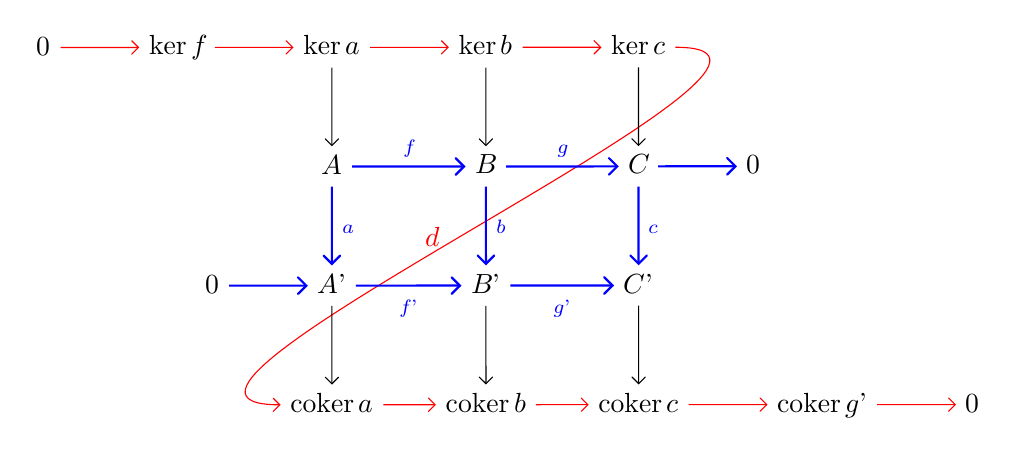
\begin{tikzpicture}[>=angle 90,scale=2.2,text height=1.5ex, text depth=0.25ex]
    %% First place the nodes
    \node (k-1) at (0,3) {$0$};
    \node (k0) [right=of k-1] {$\ker f$};
    \node (k1) [right=of k0] {$\ker a$};
    \node (k2) [right=of k1] {$\ker b$};
    \node (k3) [right=of k2] {$\ker c$};
    \node (a1) [below=of k1] {$A$};
    \node (a2) [below=of k2] {$B$};
    \node (a3) [below=of k3] {$C$};
    \node (a4) [right=of a3] {$0$};
    \node (b1) [below=of a1] {$A’$};
    \node (b0) [left=of b1] {$0$};
    \node (b2) [below=of a2] {$B’$};
    \node (b3) [below=of a3] {$C’$};
    \node (c1) [below=of b1] {$\coker a$};
    \node (c2) [below=of b2] {$\coker b$};
    \node (c3) [below=of b3] {$\coker c$};
    \node (c4) [right=of c3] {$\coker g’$};
    \node (c5) [right=of c4] {$0$};
    %% Draw the red arrows
    \draw[->,red,font=\scriptsize]
    (k-1) edge (k0)
    (k0) edge (k1)
    (k1) edge (k2)
    (k2) edge (k3)
    (c1) edge (c2)
    (c2) edge (c3)
    (c3) edge (c4)
    (c4) edge (c5);
    %% Draw the curvy red arrow
    \draw[->,red]
    (k3) edge[out=0,in=180,red] node[pos=0.55,yshift=5pt] {$d$} (c1);
    %% Draw the black arrows
    \draw[->]
    (k1) edge (a1)
    (k2) edge (a2)
    (k3) edge (a3)
    (b1) edge (c1)
    (b2) edge (c2)
    (b3) edge (c3);
    %% Draw the thick blue arrows
    \draw[->,font=\scriptsize,blue,thick]
    (a1) edge node[auto] {$f$} (a2)
    (a2) edge node[auto] {$g$} (a3)
    (a3) edge (a4)
    (a1) edge node[auto] {$a$} (b1)
    (a2) edge node[auto] {$b$} (b2)
    (a3) edge node[auto] {$c$} (b3)
    (b0) edge (b1)
    (b1) edge node[below] {$f’$} (b2)
    (b2) edge node[below] {$g’$} (b3);
  \end{tikzpicture}\end{center}

Let \(C\) be a class of \(A\)-modules and let \(\lambda\) be a function on \(C\) with values in \(\Z\) (or,
more generally, with values in an abelian group \(G\)). The function \(\lambda\) is \textbf{additive} if, for each
short exact sequence in which all the terms belongs to \(C\), we have \(\lambda(M')-\lambda(M)+\lambda(M'')=0\)

\begin{examplle}[]
Let \(A\) be a field \(k\), and let \(C\) be the class of all finite-dimensional \(k\)-vector
spaces \(V\). Then \(V\mapsto\dim V\) is an additive function on \(V\)
\end{examplle}

\begin{proposition}[]
Let \(0\to M_0\to M_1\to\cdots\to M_n\to 0\) be an exact sequence of \(A\)-modules where all the modules \(M_i\)
and the kernels of all the homomorphisms belong to \(C\). Then for any additive function \(\lambda\)
on \(C\) we have
\begin{equation*}
\sum_{i=0}^n(-1)^i\lambda(M_i)=0
\end{equation*}
\end{proposition}

\begin{proof}
Split up the sequence into short exact sequences
\begin{equation*}
0\to N_i\to M_i\to N_{i+1}\to 0
\end{equation*}
(\(N_0=N_{n+1}=0\) and \(\lambda(M_0)=\lambda(M_n)=2\lambda(0)\)). Then we have \(\lambda(M_i)=\lambda(N_i)+\lambda(N_{i+1})\).
\end{proof}

Let \(M,N,P\) be three \(A\)-modules. A mapping \(f:M\times N\to P\) is said to be \textbf{\(A\)-bilinear} if
for each \(x\in M\) the mapping \(y\mapsto f(x,y)\) of \(N\) into \(P\) is \(A\)-linear, and for
each \(y\in N\) the mapping \(x\mapsto f(x,y)\) of \(M\) into \(P\) is \(A\)-linear

We shall construct an \(A\)-module \(T\), called the \textbf{tensor product} of \(M\) and \(N\), with the
property that the \(A\)-bilinear mappings \(M\times N\to P\) are in a natural one-to-one correspondence
with the \(A\)-linear mappings \(T\to P\), for all \(A\)-modules \(P\). More precisely:

\begin{proposition}[]
Let \(M,N\) be \(A\)-modules. Then there exists a pair \((T,g)\) consisting of
an \(A\)-module \(T\) and an \(A\)-bilinear mapping \(g:M\times N\to T\), with the following property:

Given any \(A\)-module \(P\) and any \(A\)-bilinear mapping \(f:M\times N\to P\), there exists a
unique \(A\)-linear mapping \(f':T\to P\) s.t. \(f=f'\circ g\)

Moreover, if \((T,g)\) and \((T',g')\) are two pairs with this property, then there is a unique
isomorphism \(j:T\to T'\) s.t. \(j\circ g=g'\)
\end{proposition}

\begin{proof}
\label{2.12}
\begin{enumerate}
\item Uniqueness. Replacing \((P,f)\) by \((T',g')\) we get a unique \(j:T\to T'\) s.t. \(g'=j\circ g\).
\item Existence. Let \(C\) denote the free \(A\)-module \(A^{(M\times N)}\). The elements of \(C\) are
formal linear combinations of elements of \(M\times N\) with coefficients in \(A\), i.e., they are
expressions of the form \(\sum_{i=1}^na_i\cdot(x_i,y_i)\) (\(a_i\in A,x_i\in M,y_i\in N\))
\wu{
here \((x_i,y_i)=(0,\dots,0,1,0,\dots,0)\) where \((x_i,y_i)\)th position is not 0 i think. And direct
sum only admits finite sum
}

Let \(D\) be the submodule of \(C\) generated by all elements of \(C\) of the following
types:
\begin{gather*}
\end{enumerate}
(x+x',y)-(x,y)-(x',y)\\
(x,y+y')-(x,y)-(x,y')\\
(ax,y)-a\(\cdot\)(x,y)\\
(x,ay)-a\(\cdot\)(x,y)
   \end{gather*}
   Let \(T=C/D\). For each basis element \((x,y)\) of \(C\), let \(x\otimes y\) denote its image
in \(T\). Then \(T\) is generated by the elements of the form \(x\otimes y\) and from our definition
we have
\begin{gather*}
(x+x')\otimes y=x\otimes y+x'\otimes y,\quad x\otimes(y+y')=x\otimes y+x\otimes y'\\
(ax)\otimes y=x\otimes (ay)=a(x\otimes y)
\end{gather*}
Equivalently, the mapping \(g:M\times N\to T\) defined by \(g(x,y)=x\otimes y\) is \(A\)-bilinear

Any map \(f\) of \(M\times N\) into an \(A\)-module \(P\) extends by linearity to an \(A\)-module
homomorphism \(\barf:C\to P\)
\wu{
\(\barf(\sum_{i=1}^na_i\cdot(x_i,y_i))=\sum_{i=1}^na_i\cdot f(x_i,y_i)\)
}
Suppose in particular that \(f\) is \(A\)-bilinear. Then, from the
definitions, \(\barf\) vanishes on all the generators of \(D\), hence on the whole of \(D\), and
therefore induces a well-defined \(A\)-homomorphism \(f'\) of \(T=C/D\) into \(P\)
s.t. \(f'(x\otimes y)=f(x,y)\)
\end{proof}

\begin{remark}
\begin{enumerate}
\item The module \(T\) constructed above is called the \textbf{tensor product} of \(M\) and \(N\), and is
denoted by \(M\otimes_AN\). It is generated as an \(A\)-module by the ``products'' \(x\otimes y\).
If \((x_i)_{i\in I},(y_i)_{j\in J}\) are families of generators of \(M,N\) respectively, then the
elements \(x_i\otimes y_j\) generated \(M\otimes N\)
\item The notation \(x\otimes y\) is inherently ambiguous unless we specify the tensor product to which
it belongs. Let \(M',N'\) be submodules of \(M,N\) respectively, and let \(x\in M'\)
and \(y\in N'\). Then it can happen that \(x\otimes y\) as an element of \(M\otimes N\) is zero
whilst \(x\otimes y\) as an element of \(M'\otimes N'\) is non-zero. For example,
take \(A=\Z,M=\Z,N=\Z/2\Z\), and let \(M'\) be the submodule \(2\Z\) of \(\Z\), whilst \(N'=N\).
Let \(x\) be the non-zero element of \(N\) and consider \(2\otimes x\). As an element
of \(M\otimes N\), it is zero because \(2\otimes x=1\otimes 2x=1\otimes 0=0\). But as an element of \(M'\otimes N'\) it is
not zero
\end{enumerate}
\end{remark}

\begin{corollary}[]
\label{2.13}
Let \(x_i\in M\), \(y_i\in N\) be s.t. \(\sum x_i\otimes y_i=0\) in \(M\otimes N\). Then there exist finitely generated
submodules \(M_0\) of \(M\) and \(N_0\) of \(N\) s.t. \(\sum x_i\otimes y_i=0\) in \(M_0\otimes N_0\)
\end{corollary}

\begin{proof}
If \(\sum x_i\otimes y_i=0\), then \(\sum(x_i,y_i)\in D\) and therefore \(\sum(x_i,y_i)\) is a finite sum of generators
of \(D\). Let \(M_0\) be the submodule of \(M\) generated by the \(x_i\) and all the elements
of \(M\) which occur as first coordinates in these generators of \(D\), and define \(N_0\)
similarly. Then \(\sum x_i\otimes y_i=0\) as an element of \(M_0\otimes N_0\)
\end{proof}


\begin{remark}
\begin{enumerate}
\setcounter{enumi}{2}
\item We shall never again need to use the construction of the tensor product given in
\ref{2.12}. What is essential to keep in mind is the defining property of the tensor product
\item Instead of starting with bilinear mappings we could have started with multilinear
mappings \(f:M_1\times\cdots\times M_r\to P\) defined in the same way.
\end{enumerate}
\end{remark}

\begin{proposition}[]
Let \(M_1,\dots,M_r\) be \(A\)-modules. Then there is a pair \((T,g)\) consisting of
an \(A\)-module \(T\) and an \(A\)-multilinear mapping \(g:M_1\times\dots\times M_r\to T\) with the following
property:

Given any \(A\)-module \(P\) and any \(A\)-multilinear mapping \(f:M_1\times\cdots\times M_r\to T\), there exists a
unique \(A\)-homomorphism \(f':T\to P\) s.t. \(f'\circ g=f\)

Moreover, if \((T,g)\) and \((T',g')\) are two pairs with this property, then there exists a
unique isomorphism \(j:T\to T'\) s.t. \(j\circ g=g'\)
\end{proposition}

\begin{proposition}[]
Let \(M,N,P\) be \(A\)-modules. Then there exist unique isomorphisms
\begin{enumerate}
\item \(M\otimes N\to N\otimes M\)
\item \((M\otimes N)\otimes P\to M\otimes(N\otimes P)\to M\otimes N\otimes P\)
\end{enumerate}


s.t., respectively
\begin{enumerate}
\item \(x\otimes y\mapsto y\otimes x\)
\item \((x\otimes y)\otimes z\mapsto x\otimes(y\otimes z)\to x\otimes y\otimes z\)
\end{enumerate}
\end{proposition}

\begin{proof}
\begin{enumerate}
\item 

\item We shall construct homomorphisms
\begin{equation*}
(M\otimes N)\otimes P\xrightarrow{f}M\otimes N\otimes P\xrightarrow{g}(M\otimes N)\otimes P
\end{equation*}
s.t. \(f((x\otimes y)\otimes z)=x\otimes y\otimes z\) and \(g(x\otimes y\otimes z)=(x\otimes y)\otimes z\) for all \(x\in M,y\in N,z\in P\)

To construct \(f\), fix the element \(z\in P\). The mapping \((x,y)\mapsto x\otimes y\otimes z\) is bilinear and
therefore induces a homomorphism \(f_z:M\otimes N\to M\otimes N\otimes P\). Next consider the
mapping \((t,z)\mapsto f_z(t)\) of \((M\otimes N)\times P\) into \(M\otimes N\otimes P\). This is bilinear in \(t\)
and \(z\) and therefore induces a homomorphism
\begin{equation*}
f:(M\otimes N)\otimes P\to M\otimes N\otimes P
\end{equation*}
s.t. \(f((x\otimes y)\otimes z)=x\otimes y\otimes z\)

To construct \(g\), consider the mapping \((x,y,z)\mapsto(x\otimes y)\otimes z\) of \(M\times N\times P\)
into \((M\otimes N)\otimes P\). This is linear in each variable and therefore induces a homomorphism
\begin{equation*}
g:M\otimes N\otimes P\to(M\otimes N)\otimes P
\end{equation*}
s.t. \(g(x\otimes y\otimes z)=(x\otimes y)\otimes z\)

Clearly \(f\circ g\) and \(g\circ f\) are identity, hence \(f\) and \(g\) are isomorphisms
\end{enumerate}
\end{proof}



\section{{\bfseries\sffamily TODO} Problems}
\label{sec:orgb8fec3e}
\ref{Problem1}: need more field knowledge to deal with \(\R[x]\) and \(\Z[x]\)

\ref{Problem2}: need more matrix

\href{https://mathoverflow.net/questions/42241/errata-for-atiyah-macdonald}{Errata}
\end{document}
